% !Mode:: "TeX:UTF-8"
\chapter{建图}
\begin{mdframed}  
	\textbf{主要目标}
	\begin{enumerate}[labelindent=0em,leftmargin=1.5em]
		\item 理解单目SLAM中稠密深度估计的原理。
		\item 通过实验了解单目稠密重建的过程。
		\item 了解几种RGB-D重建中的地图形式。
	\end{enumerate}
\end{mdframed}

本讲我们开始介绍建图部分的算法。在前端和后端中,我们重点关注同时估计相机运动轨迹与特征点空间位置的问题。然而,在实际使用SLAM时,除了对相机本体进行定位之外,还存在许多其他的需求。例如,考虑放在机器人上的SLAM,那么我们会希望地图能够用于定位、导航、避障和交互,特征点地图显然不能满足所有的这些需求。所以,本讲我们将更详细地讨论各种形式的地图,并指出目前视觉SLAM地图中存在着的缺陷。

\newpage
\section{概述}
建图(Mapping),本应该是SLAM的两大目标之一——因为SLAM被称为同时定位与建图。但是直到现在,我们讨论的都是定位问题,包括通过特征点的定位、直接法的定位,以及后端优化。那么,这是否暗示建图在SLAM里没有那么重要,所以我们直到本讲才开始讨论呢?

答案是否定的。事实上,在经典的SLAM模型中,我们所谓的地图,即所有路标点的集合。一旦确定了路标点的位置,那就可以说我们完成了建图。于是,前面说的视觉里程计也好,Bundle Adjustment也好,事实上都建模了路标点的位置,并对它们进行优化。从这个角度上说,我们已经探讨了建图问题。那么为何还要单独列一讲建图呢?

这是因为人们对建图的需求不同。SLAM作为一种底层技术,往往是用来为上层应用提供信息的。如果上层是机器人,那么应用层的开发者可能希望使用SLAM来做全局的定位,并且让机器人在地图中导航——例如扫地机需要完成扫地工作,希望计算一条能够覆盖整张地图的路径。或者,如果上层是一个增强现实设备,那么开发者可能希望将虚拟物体叠加在现实物体之中,特别地,还可能需要处理虚拟物体和真实物体的遮挡关系。

我们发现,应用层面对于“定位”的需求是相似的,它们希望SLAM提供相机或搭载相机的主体的空间位姿信息。而对于地图,则存在着许多不同的需求。在视觉SLAM看来,“建图”是服务于“定位”的;但是在应用层面看来,“建图”明显还带有许多其他的需求。关于地图的用处,我们大致归纳如下:

\begin{enumerate}
	\item \textbf{定位}。定位是地图的一项基本功能。在前面的视觉里程计部分,我们讨论了如何利用局部地图来实现定位。在回环检测部分,我们也看到,只要有全局的描述子信息,我们也能通过回环检测确定机器人的位置。更进一步,我们还希望能够把地图保存下来,让机器人在下次开机后依然能在地图中定位,这样只需对地图进行一次建模,而不是每次启动机器人都重新做一次完整的SLAM。
	\item \textbf{导航}。导航是指机器人能够在地图中进行路径规划,在任意两个地图点间寻找路径,然后控制自己运动到目标点的过程。该过程中,我们至少需要知道\textbf{地图中哪些地方不可通过,而哪些地方是可以通过的}。这就超出了稀疏特征点地图的能力范围,我们必须有另外的地图形式。稍后我们会说,这至少得是一种\textbf{稠密}的地图。
	\item \textbf{避障}。避障也是机器人经常碰到的一个问题。它与导航类似,但更注重局部的、动态的障碍物的处理。同样,仅有特征点,我们无法判断某个特征点是否为障碍物,所以需要\textbf{稠密}地图。
	\item \textbf{重建}。有时候,我们希望利用SLAM获得周围环境的重建效果。这种地图主要用于向人展示,所以我们希望它看上去比较舒服、美观。或者,我们也可以把该地图用于通信,使其他人能够远程地观看我们重建得到的三维物体或场景——例如三维的视频通话或者网上购物等。这种地图亦是\textbf{稠密}的,并且我们还对它的外观有一些要求。我们可能不满足于稠密点云重建,更希望能够构建带纹理的平面,就像电子游戏中的三维场景那样。
	\item \textbf{交互}。交互主要指人与地图之间的互动。例如,在增强现实中,我们会在房间里放置虚拟的物体,并与这些虚拟物体之间有一些互动——比方说我会点击墙面上放着的虚拟网页浏览器来观看视频,或者向墙面投掷物体,希望它们有(虚拟的)物理碰撞。另一方面,机器人应用中也会有与人、与地图之间的交互。例如,机器人可能会收到命令“取桌子上的报纸”,那么,除了有环境地图之外,机器人还需要知道哪一块地图是“桌子”,什么叫作“之上”,什么又叫作“报纸”。这需要机器人对地图有更高层面的认知——亦称为语义地图。
\end{enumerate}

\autoref{fig:maps}~形象地解释了上面讨论的各种地图类型与用途之间的关系。我们之前的讨论,基本集中于“稀疏路标地图”部分,还没有探讨稠密地图。所谓稠密地图是相对于稀疏地图而言的。稀疏地图只建模感兴趣的部分,也就是前面说了很久的特征点(路标点)。而稠密地图是指,建模\textbf{所有}看到过的部分。对于同一张桌子,稀疏地图可能只建模了桌子的四个角,而稠密地图则会建模整个桌面。虽然从定位角度看,只有四个角的地图也可以用于对相机进行定位,但由于我们无法从四个角推断这几个点之间的空间结构,所以无法仅用四个角来完成导航、避障等需要稠密地图才能完成的工作。

\begin{figure}[!ht]
	\centering
	\includegraphics[width=1.0\textwidth]{mapping/maps.pdf}
	\caption{各种地图的示意图。三种例子地图分别来自文献\cite{Mur-Artal2015, Labbe2014, Salas-Moreno2013}。}
	\label{fig:maps}
\end{figure}

从上面的讨论中可以看出,稠密地图占据着一个非常重要的位置。于是,剩下的问题是:通过视觉SLAM能建立稠密地图吗?如果能,怎么建呢?

\section{单目稠密重建}
\subsection{立体视觉}
视觉SLAM的稠密重建问题是本讲的第一个重要话题。相机,很久以来被认为是只有角度的传感器(Bearing only)。单幅图像中的像素,只能提供物体与相机成像平面的角度及物体采集到的亮度,而无法提供物体的距离(Range)。而在稠密重建中,我们需要知道每一个像素点(或大部分像素点)的距离,对此大致上有如下解决方案:

\begin{enumerate}
	\item 使用单目相机,通过移动相机之后进行三角化测量像素的距离。
	\item 使用双目相机,利用左右目的视差计算像素的距离(多目原理相同)。
	\item 使用RGB-D相机直接获得像素距离。
\end{enumerate}

前两种方式称为立体视觉(Stereo Vision),其中移动单目的又称为移动视角的立体视觉(Moving View Stereo)。相比于RGB-D直接测量的深度,单目和双目对深度的获取往往是“费力不讨好”的——我们需要花费大量的计算,最后得到一些不怎么可靠的\footnote{正式点叫Fragile。}深度估计。当然,RGB-D也有一些量程、应用范围和光照的限制,不过相比于单目和双目的结果,使用RGB-D进行稠密重建往往是更常见的选择。而单目、双目的好处是,在目前RGB-D还无法很好应用的室外、大场景场合中,仍能通过立体视觉估计深度信息。

话虽如此,本节我们将带领读者实现一遍单目的稠密估计,体验为何说它是费力不讨好的。我们从最简单的情况开始说起:在给定相机轨迹的基础上,如何根据一段时间的视频序列来估计某幅图像的深度。换言之,我们不考虑SLAM,先来考虑略为简单的建图问题。

假定有一段视频序列,我们通过某种魔法得到了每一帧对应的轨迹(当然也很可能是由视觉里程计前端估计所得)。现在我们以第一幅图像为参考帧,计算参考帧中每一个像素的深度(或者说距离)。首先,请回忆在特征点部分我们是如何完成该过程的:

\begin{enumerate}
	\item 首先,我们对图像提取特征,并根据描述子计算了特征之间的匹配。换言之,通过特征,我们对某一个空间点进行了跟踪,知道了它在各个图像之间的位置。
	\item 然后,由于我们无法仅用一幅图像确定特征点的位置,所以必须通过不同视角下的观测估计它的深度,原理即前面讲过的三角测量。
\end{enumerate}

在稠密深度图估计中,不同之处在于,我们无法把每个像素都当作特征点计算描述子。因此,稠密深度估计问题中,匹配就成为很重要的一环:如何确定第一幅图的某像素出现在其他图里的位置呢?这需要用到\textbf{极线搜索}和\textbf{块匹配技术}\textsuperscript{\cite{Pizzoli2014}}。然后,当我们知道了某个像素在各个图中的位置,就能像特征点那样,利用三角测量确定它的深度。不过不同的是,在这里我们要使用很多次三角测量让深度估计收敛,而不仅是一次。我们希望深度估计能够随着测量的增加从一个非常不确定的量,逐渐收敛到一个稳定值。这就是\textbf{深度滤波器技术}。所以,下面的内容将主要围绕这个主题展开。

\subsection{极线搜索与块匹配}

我们先来探讨不同视角下观察同一个点产生的几何关系。这非常像在第~\ref{sec:epipolar-geometry}~节讨论的对极几何关系。请看\autoref{fig:epipolar-line-search}~。左边的相机观测到了某个像素$\bm{p}_1$。由于这是一个单目相机,我们无从知道它的深度,所以假设这个深度可能在某个区域之内,不妨说是某最小值到无穷远之间:$(d_\mathrm{min}, +\infty)$。因此,该像素对应的空间点就分布在某条线段(本例中是射线)上。在另一个视角(右侧相机)看来,这条线段的投影也形成图像平面上的一条线,我们知道这称为\textbf{极线}。当知道两部相机间的运动时,这条极线也是能够确定的\footnote{反之,如果运动不知道,那么极线也无法确定。}。那么问题就是:极线上的哪一个点是我们刚才看到的$\bm{p}_1$点呢?

\begin{figure}[!htp]
	\centering
	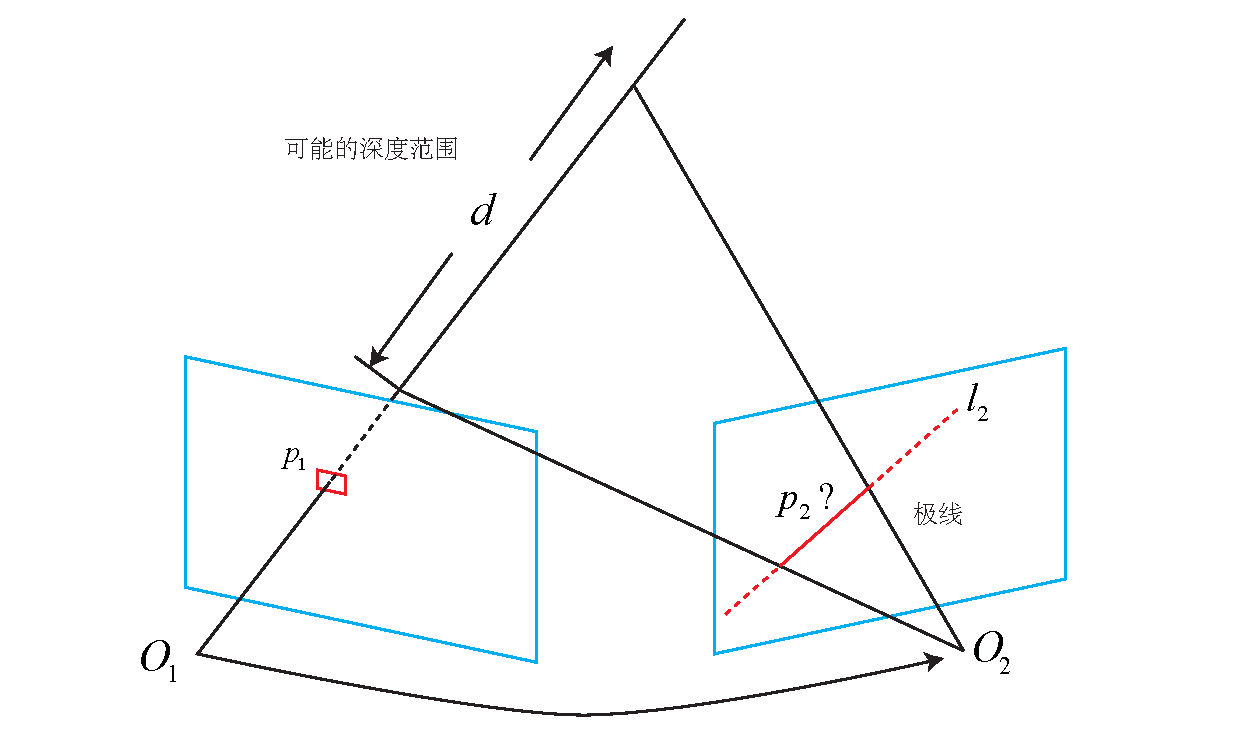
\includegraphics[width=.8\textwidth]{mapping/epipolar-line-search.pdf}
	\caption{极线搜索示意图。}
	\label{fig:epipolar-line-search}
\end{figure}

重复一遍,在特征点方法中,我们通过特征匹配找到了$\bm{p}_2$的位置。然而现在我们没有描述子,所以只能在极线上搜索和$\bm{p}_1$长得比较相似的点。再具体地说,我们可能沿着第二幅图像中的极线的某一头走到另一头,逐个比较每个像素与$\bm{p}_1$的相似程度。从直接比较像素的角度来看,这种做法倒是和直接法是异曲同工的。

在直接法的讨论中我们知道,比较单个像素的亮度值并不一定稳定可靠。一件很明显的事情就是:万一极线上有很多和$\bm{p}_1$相似的点,我们怎么确定哪一个是真实的呢?这似乎回到了我们在回环检测当中说到的问题:如何确定两幅图像(或两个点)的相似性?回环检测是通过词袋来解决的,但这里由于没有特征,所以只好寻求另外的途径。

一种直观的想法是:既然单个像素的亮度没有区分性,那是否可以比较像素块呢?我们在$\bm{p}_1$周围取一个大小为$w \times w$的小块,然后在极线上也取很多同样大小的小块进行比较,就可以在一定程度上提高区分性。这就是所谓的\textbf{块匹配}。注意到在这个过程中,只有假设在不同图像间整个小块的灰度值不变,这种比较才有意义。所以算法的假设,从像素的灰度不变性,变成了图像块的灰度不变性——在一定程度上变得更强了。

好了,现在我们取了$\bm{p}_1$周围的小块,并且在极线上也取了很多个小块。不妨把$\bm{p}_1$周围的小块记成$\bm{A} \in \mathbb{R}^{w \times w}$,把极线上的$n$个小块记成$\bm{B}_i, i=1, \cdots, n$。那么,如何计算小块与小块间的差异呢?有若干种不同的计算方法:

\begin{enumerate}
	\item SAD(Sum of Absolute Difference)。顾名思义,即取两个小块的差的绝对值之和:
	\begin{equation}
	S( \bm{A}, \bm{B} )_{\mathrm{SAD}} = \sum_{i,j} | \bm{A}(i,j) - \bm{B}(i,j) |.
	\end{equation}
	\item SSD。这里的SSD并不是指大家熟悉的固态硬盘,而是Sum of Squared Distance(平方和)的意思:
	\begin{equation}
	S( \bm{A}, \bm{B} )_{\mathrm{SSD}} = \sum_{i,j} \left( \bm{A}(i,j) - \bm{B}(i,j) \right)^2.
	\end{equation}
	\item NCC(Normalized Cross Correlation,归一化互相关)。这种方式比前两种要复杂一些,它计算的是两个小块的相关性:
	\begin{equation}
	S( \bm{A}, \bm{B} )_{\mathrm{NCC}} = \frac{{\sum\limits_{i,j} {\bm{A}(i,j)\bm{B}(i,j)} }}{{\sqrt {\sum\limits_{i,j} {\bm{A}{{(i,j)}^2}\sum\limits_{i,j} {\bm{B}{{(i,j)}^2}} } } }}.
	\end{equation}
	请注意,由于这里用的是相关性,所以相关性接近0表示两幅图像不相似,而接近1才表示相似。前面两种距离则是反过来的,接近0表示相似,而大的数值表示不相似。
\end{enumerate}

和我们遇到过的许多情形一样,这些计算方式往往存在一个精度−效率之间的矛盾。精度好的方法往往需要复杂的计算,而简单的快速算法又往往效果不佳。这需要我们在实际工程中进行取舍。另外,除了这些简单版本之外,我们可以\textbf{先把每个小块的均值去掉},称为去均值的SSD、去均值的NCC,等等。去掉均值之后,我们允许像“小块$\bm{B}$比$\bm{A}$整体上亮一些,但仍然很相似”这样的情况\footnote{整体亮一些可能由环境光照变亮或相机曝光参数升高导致。},因此比之前的更加可靠一些。如果读者对更多的块匹配度量方法感兴趣,建议阅读文献\cite{stereo-matching-website, Hirschmuller2007}作为补充材料。

现在,我们在极线上计算了$\bm{A}$与每一个$\bm{B}_i$的相似性度量。为了方便叙述,假设我们用了NCC,那么,我们将得到一个沿着极线的NCC分布。这个分布的形状严重取决于图像本身的样子,如\autoref{fig:matching-score}~所示。在搜索距离较长的情况下,我们通常会得到一个非凸函数:这个分布存在着许多峰值,然而真实的对应点必定只有一个。在这种情况下,我们会倾向于使用概率分布来描述深度值,而非用某个单一的数值来描述深度。于是,我们的问题就转到了在不断对不同图像进行极线搜索时,我们估计的深度分布将发生怎样的变化——这就是所谓的\textbf{深度滤波器}。

\begin{figure}[!htp]
	\centering
	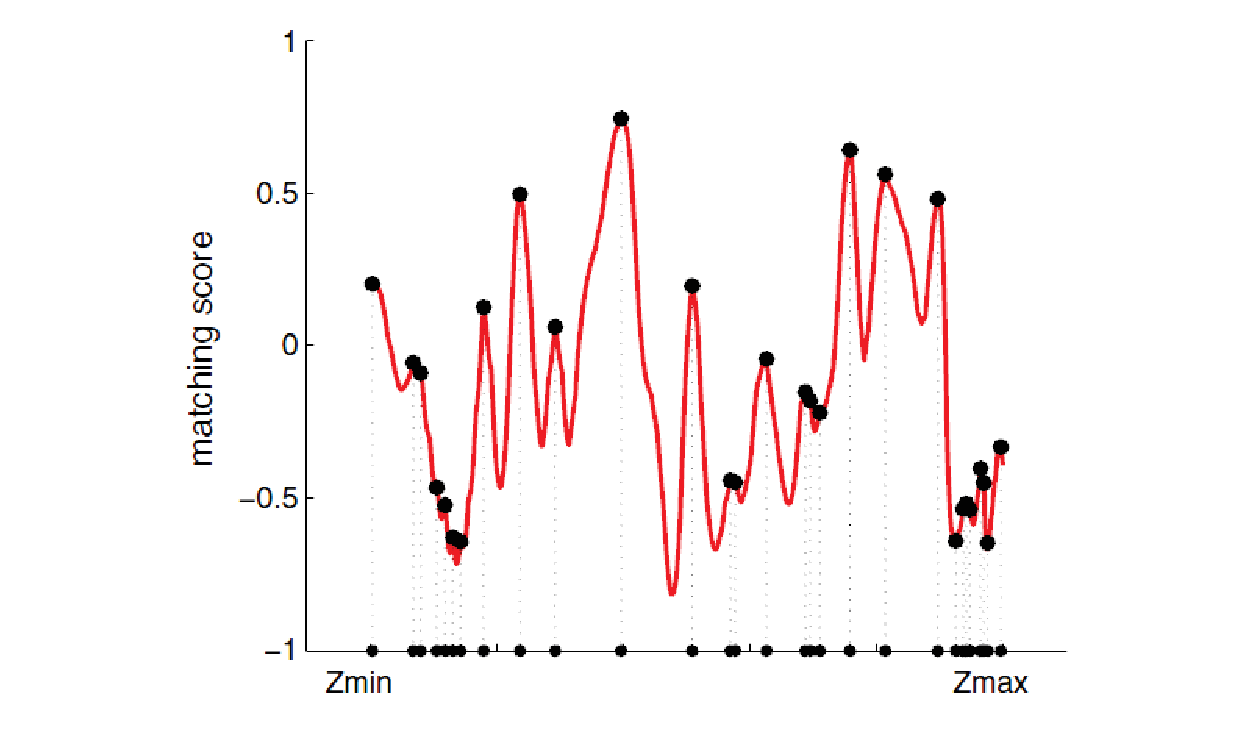
\includegraphics[width=.75\textwidth]{mapping/matching-score.pdf}
	\caption{匹配得分沿距离的分布,图像来自文献\cite{Vogiatzis2011}。}
	\label{fig:matching-score}
\end{figure}

\subsection{高斯分布的深度滤波器}
对像素点深度的估计,本身亦可建模为一个状态估计问题,于是就自然存在滤波器与非线性优化两种求解思路。虽然非线性优化效果较好,但是在SLAM这种实时性要求较强的场合,考虑到前端已经占据了不少的计算量,建图方面则通常采用计算量较少的滤波器方式了。这也是本节讨论深度滤波器的目的。

对深度的分布假设存在着若干种不同的做法。首先,在比较简单的假设条件下,我们可以假设深度值服从高斯分布,得到一种类卡尔曼式的方法(但实际上只是归一化积,我们稍后会看到)。而另一方面,在\cite{Vogiatzis2011, Forster2014}等文献中,亦采用了均匀−高斯混合分布的假设,推导了另一种形式更为复杂的深度滤波器。本着简单易用的原则,我们先来介绍并演示高斯分布假设下的深度滤波器,然后把均匀−高斯混合分布的滤波器作为习题。

设某个像素点的深度$d$服从:
\begin{equation}
P(d) = N(\mu, \sigma^2).
\end{equation}

而每当新的数据到来,我们都会观测到它的深度。同样,假设这次观测亦是一个高斯分布:
\begin{equation}
P(d_{\mathrm{obs}}) = N(\mu_{\mathrm{obs}}, \sigma_{\mathrm{obs}}^2 ).
\end{equation}

于是,我们的问题是,如何使用观测的信息更新原先$d$的分布。这正是一个信息融合问题。根据附录A,我们明白两个高斯分布的乘积依然是一个高斯分布。设融合后的$d$的分布为$N(\mu_{\mathrm{fuse}}, \sigma_{\mathrm{fuse}}^2)$,那么根据高斯分布的乘积,有:
\begin{equation}
{\mu _{\mathrm{fuse}}} = \frac{{\sigma _{\mathrm{obs}}^2\mu  + {\sigma ^2}{\mu _{\mathrm{obs}}}}}{{{\sigma ^2} + \sigma _{\mathrm{obs}}^2}},\quad \sigma _{\mathrm{fuse}}^2 = \frac{{{\sigma ^2}\sigma _{\mathrm{obs}}^2}}{{{\sigma ^2} + \sigma _{\mathrm{obs}}^2}}.
\end{equation}

由于我们仅有观测方程而没有运动方程,所以这里深度仅用到了信息融合部分,而无须像完整的卡尔曼那样进行预测和更新。可以看到融合的方程确实比较浅显易懂,不过问题仍然存在:如何确定我们观测到深度的分布呢?即,如何计算$\mu_{\mathrm{obs}}, \sigma_{\mathrm{obs}}$呢?

关于$\mu_{\mathrm{obs}}, \sigma_{\mathrm{obs}}$,亦存在一些不同的处理方式。例如,文献\cite{Engel2013}考虑了几何不确定性和光度不确定性二者之和,而\cite{Vogiatzis2011}则仅考虑了几何不确定性。我们暂时只考虑由几何关系带来的不确定性。现在,假设我们通过极线搜索和块匹配确定了参考帧某个像素在当前帧的投影位置。那么,这个位置对深度的不确定性有多大呢?

以\autoref{fig:uncertainty-mapping}~为例。考虑某次极线搜索,我们找到了$\bm{p}_1$对应的$\bm{p}_2$点,从而观测到了$\bm{p}_1$的深度值,认为$\bm{p}_1$对应的三维点为$\bm{P}$。从而,可记$\bm{O}_1 \bm{P}$为$\bm{p}$,$\bm{O}_1 \bm{O}_2$为相机的平移$\bm{t}$,$\bm{O}_2 \bm{P}$记为$\bm{a}$。并且,把这个三角形的下面两个角记作$\alpha, \beta$。现在,考虑极线$l_2$上存在着一个像素大小的误差,使得$\beta$角变成了$\beta'$,而$\bm{p}_2$也变成了$\bm{p}_2'$,并记上面那个角为$\gamma$。 我们要问的是,这一个像素的误差会导致$\bm{p}'$与$\bm{p}$产生多大的差距呢?

\begin{figure}[!ht]
	\centering
	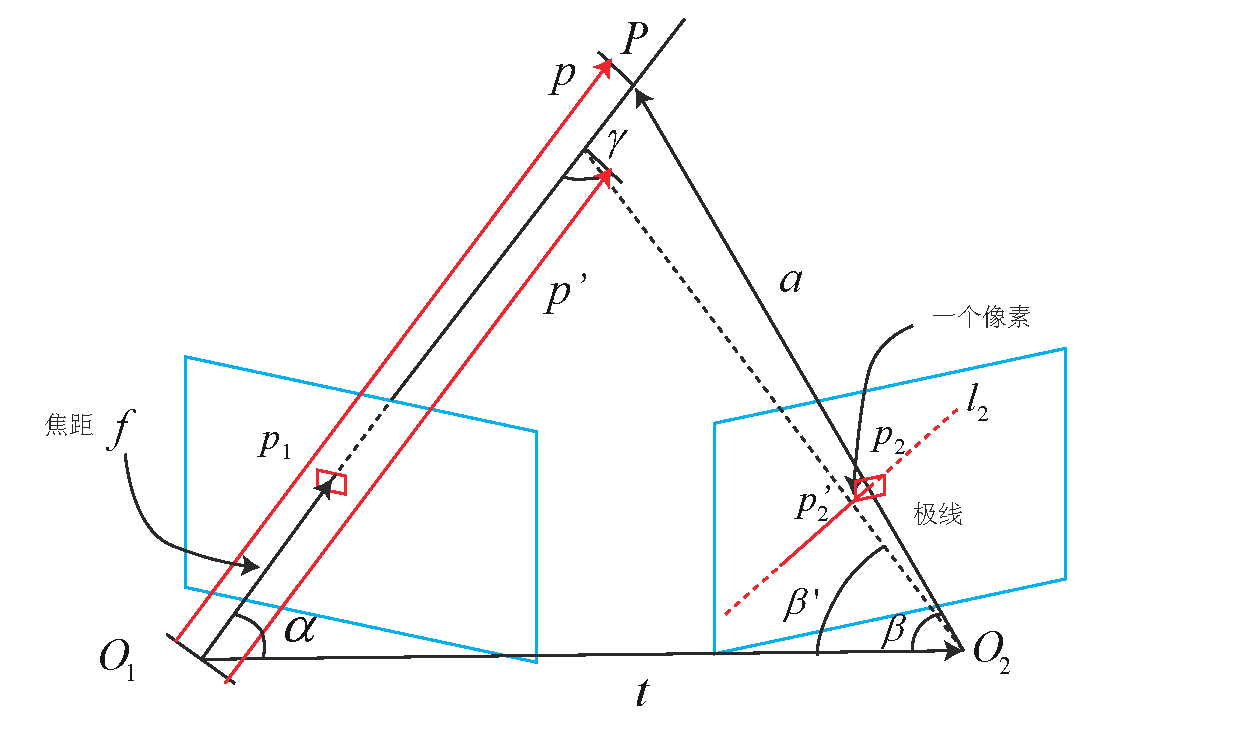
\includegraphics[width=.84\textwidth]{mapping/uncertainty.pdf}
	\caption{不确定性分析。}
	\label{fig:uncertainty-mapping}
\end{figure}

这是一个典型的几何问题。我们来列写这些量之间的几何关系。显然有:
\begin{equation}
\begin{array}{l}
\bm{a} = \bm{p} - \bm{t} \\
\alpha  = \arccos \left\langle {\bm{p}, \bm{t}} \right\rangle \\
\beta  = \arccos \left\langle {\bm{a}, - \bm{t}} \right\rangle .
\end{array}
\end{equation}

对$\bm{p}_2$扰动一个像素,将使得$\beta$产生一个变化量,成为$\beta '$。根据几何关系,有:
\begin{equation}
\begin{array}{l}
\beta ' = \arccos \left\langle {\bm{O}_2 \bm{p}_2', -\bm{t}} \right\rangle \\
\gamma  = \pi  - \alpha  - \beta '.
\end{array}
\end{equation}

于是,由正弦定理,$\bm{p}'$的大小可以求得:
\begin{equation}
\| \bm{p}' \| = \| \bm{t} \| \frac{{\sin \beta '}}{{\sin \gamma }}.
\end{equation}

由此,我们确定了由单个像素的不确定引起的深度不确定性。如果认为极线搜索的块匹配仅有一个像素的误差,那么就可以设:
\begin{equation}
\sigma_{\mathrm{obs}} = \| \bm{p} \|-\| \bm{p}' \|.
\end{equation}

当然,如果极线搜索的不确定性大于一个像素,我们亦可按照此推导来放大这个不确定性。接下来的深度数据融合,已经在前面介绍过了。在实际工程中,当不确定性小于一定阈值之后,就可以认为深度数据已经收敛了。

综上所述,我们给出了估计稠密深度的一个完整的过程:
\begin{mdframed}
\begin{enumerate}
	\item 假设所有像素的深度满足某个初始的高斯分布。
	\item 当新数据产生时,通过极线搜索和块匹配确定投影点位置。
	\item 根据几何关系计算三角化后的深度及不确定性。
	\item 将当前观测融合进上一次的估计中。若收敛则停止计算,否则返回第2步。
\end{enumerate}
\end{mdframed}

这些步骤组成了一套可行的深度估计方式。请注意这里说的深度值是$O_1 P$的长度,它和我们在针孔相机模型里提到的“深度”有一些少许不同——针孔相机中的深度是指像素的$z$值。我们将在实践部分进行演示该算法的结果。

\section{实践:单目稠密重建}
本节的示例程序将使用REMODE\textsuperscript{\cite{Handa2012, Pizzoli2014}}的测试数据集。它提供了一架无人机采集的单目俯视图像,共有200张,同时提供了每张图像的真实位姿。下面我们来考虑,在这些数据的基础上估算第一帧图像每个像素对应的深度值,即进行单目稠密重建。

首先,请读者从~\url{http://rpg.ifi.uzh.ch/datasets/remode_test_data.zip}~处下载示例程序所用的数据。你可以使用网页浏览器或下载工具进行下载。解压后,将在test\_data/Images中发现从0至200的所有图像,并在test\_data目录下看到一个文本文件,它记录了每幅图像对应的位姿:
\begin{lstlisting}
scene_000.png 1.086410 4.766730 -1.449960 0.789455 0.051299 -0.000779 0.611661
scene_001.png 1.086390 4.766370 -1.449530 0.789180 0.051881 -0.001131 0.611966
scene_002.png 1.086120 4.765520 -1.449090 0.788982 0.052159 -0.000735 0.612198
......
\end{lstlisting}

\autoref{fig:remode-dataset}~展示了若干时刻的图像。可以看到场景主要由地面、桌子及桌子上的杂物组成。如果深度估计大致正确,那么我们至少可以看出桌子与地面的深度值不同之处。下面,我们按照之前的讲解书写稠密深度估计程序。为了方便理解,程序书写成了C语言风格,放在单个文件中。本程序稍微有点长,在书中重点讲解几个重要函数,其余内容请读者对照GitHub的源码进行阅读。

\begin{figure}[!ht]
	\centering
	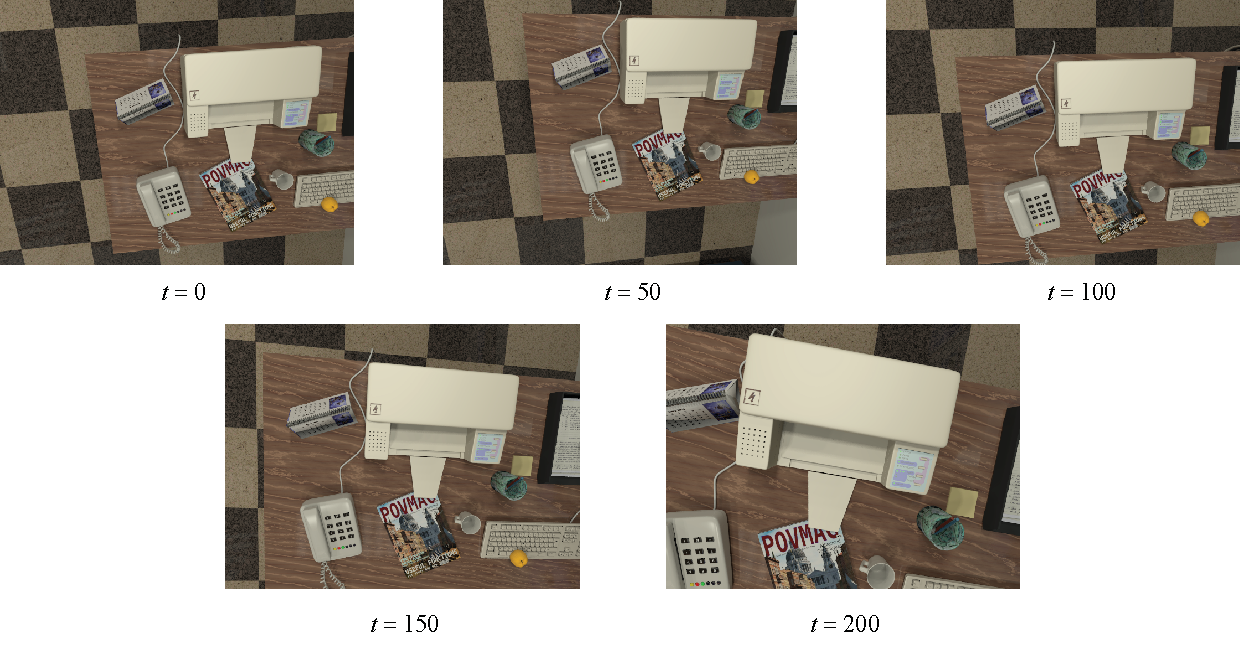
\includegraphics[width=1.0\textwidth]{mapping/remode-dataset.pdf}
	\caption{数据集图示。}
	\label{fig:remode-dataset}
\end{figure}

\begin{lstlisting}[language=c++,caption=slambook/ch13/dense\_monocular/dense\_mapping.cpp(片段)]
#include <iostream>
#include <vector>
#include <fstream>
using namespace std; 
#include <boost/timer.hpp>

// for sophus 
#include <sophus/se3.h>
using Sophus::SE3;

// for eigen 
#include <Eigen/Core>
#include <Eigen/Geometry>
using namespace Eigen;

#include <opencv2/core/core.hpp>
#include <opencv2/highgui/highgui.hpp>
#include <opencv2/imgproc/imgproc.hpp>

using namespace cv;

/**********************************************
* 本程序演示了单目相机在已知轨迹下的稠密深度估计
* 使用极线搜索 + NCC匹配的方式,与本书13.2节对应
* 请注意,本程序并不完美,你完全可以改进它。
***********************************************/

// ------------------------------------------------------------------
// parameters 
const int boarder = 20; 	// 边缘宽度
const int width = 640;  	// 宽度
const int height = 480;  	// 高度
const double fx = 481.2f;	// 相机内参
const double fy = -480.0f;
const double cx = 319.5f;
const double cy = 239.5f;
const int ncc_window_size = 2;	// NCC 取的窗口半宽度
const int ncc_area = (2*ncc_window_size+1)*(2*ncc_window_size+1); // NCC窗口面积
const double min_cov = 0.1;	// 收敛判定:最小方差
const double max_cov = 10;	// 发散判定:最大方差

// ------------------------------------------------------------------
// 重要的函数 
// 从 REMODE 数据集读取数据  
bool readDatasetFiles( 
	const string& path, 
	vector<string>& color_image_files, 
	vector<SE3>& poses 
);

// 根据新的图像更新深度估计
bool update( 
	const Mat& ref, 
	const Mat& curr, 
	const SE3& T_C_R, 
	Mat& depth, 
	Mat& depth_cov 
);

// 极线搜索 
bool epipolarSearch( 
	const Mat& ref, 
	const Mat& curr, 
	const SE3& T_C_R, 
	const Vector2d& pt_ref, 
	const double& depth_mu, 
	const double& depth_cov,
	Vector2d& pt_curr
);

// 更新深度滤波器 
bool updateDepthFilter( 
	const Vector2d& pt_ref, 
	const Vector2d& pt_curr, 
	const SE3& T_C_R, 
	Mat& depth, 
	Mat& depth_cov
);

// 计算 NCC 评分 
double NCC( const Mat& ref, const Mat& curr, const Vector2d& pt_ref, const Vector2d& pt_curr );

// 双线性灰度插值 
inline double getBilinearInterpolatedValue( const Mat& img, const Vector2d& pt ) {
	uchar* d = & img.data[ int(pt(1,0))*img.step+int(pt(0,0)) ];
	double xx = pt(0,0) - floor(pt(0,0)); 
	double yy = pt(1,0) - floor(pt(1,0));
	return  (( 1-xx ) * ( 1-yy ) * double(d[0]) +
		xx* ( 1-yy ) * double(d[1]) +
		( 1-xx ) *yy* double(d[img.step]) +
		xx*yy*double(d[img.step+1]))/255.0;
}

// ------------------------------------------------------------------
// 一些小工具 
// 显示估计的深度图 
bool plotDepth( const Mat& depth );

// 像素到相机坐标系 
inline Vector3d px2cam ( const Vector2d px ) {
	return Vector3d ( 
		(px(0,0) - cx)/fx,
		(px(1,0) - cy)/fy, 
		1
	);
}

// 相机坐标系到像素 
inline Vector2d cam2px ( const Vector3d p_cam ) {
	return Vector2d (
		p_cam(0,0)*fx/p_cam(2,0) + cx, 
		p_cam(1,0)*fy/p_cam(2,0) + cy 
	);
}

// 检测一个点是否在图像边框内
inline bool inside( const Vector2d& pt ) {
	return pt(0,0) >= boarder && pt(1,0)>=boarder 
		&& pt(0,0)+boarder<width && pt(1,0)+boarder<=height;
}

int main( int argc, char** argv )
{
	if ( argc != 2 )
	{
		cout<<"Usage: dense_mapping path_to_test_dataset"<<endl;
		return -1;
	}

	// 从数据集读取数据
	vector<string> color_image_files; 
	vector<SE3> poses_TWC;
	bool ret = readDatasetFiles( argv[1], color_image_files, poses_TWC );
	if ( ret==false )
	{
		cout<<"Reading image files failed!"<<endl;
		return -1; 
	}
	cout<<"read total "<<color_image_files.size()<<" files."<<endl;

	// 第一张图
	Mat ref = imread( color_image_files[0], 0 );      // gray-scale image 
	SE3 pose_ref_TWC = poses_TWC[0];
	double init_depth   = 3.0;    // 深度初始值
	double init_cov2    = 3.0;    // 方差初始值 
	Mat depth( height, width, CV_64F, init_depth );         // 深度图
	Mat depth_cov( height, width, CV_64F, init_cov2 );      // 深度图方差 
	
	for ( int index=1; index<color_image_files.size(); index++ )
	{
		cout<<"*** loop "<<index<<" ***"<<endl;
		Mat curr = imread( color_image_files[index], 0 );       
		if (curr.data == nullptr) continue;
		SE3 pose_curr_TWC = poses_TWC[index];
		SE3 pose_T_C_R = pose_curr_TWC.inverse() * pose_ref_TWC;
		    // 坐标转换关系: T_C_W * T_W_R = T_C_R 
		update( ref, curr, pose_T_C_R, depth, depth_cov );
		plotDepth( depth );
		imshow("image", curr);
		waitKey(1);
	}

	
	return 0;
}

// 对整个深度图进行更新
bool update(const Mat& ref, const Mat& curr, const SE3& T_C_R, Mat& depth, Mat& depth_cov )
{
#pragma omp parallel for
	for ( int x=boarder; x<width-boarder; x++ )
#pragma omp parallel for
		for ( int y=boarder; y<height-boarder; y++ )
		{
			// 遍历每个像素
			if ( depth_cov.ptr<double>(y)[x] < min_cov 
				|| depth_cov.ptr<double>(y)[x] > max_cov ) // 深度已收敛或发散
				continue;
			// 在极线上搜索 (x,y) 的匹配 
			Vector2d pt_curr; 
			bool ret = epipolarSearch ( 
				ref, 
				curr, 
				T_C_R, 
				Vector2d(x,y), 
				depth.ptr<double>(y)[x], 
				sqrt(depth_cov.ptr<double>(y)[x]),
				pt_curr
			);
			
			if ( ret == false ) // 匹配失败
				continue; 
			
			// 取消该注释以显示匹配
			// showEpipolarMatch( ref, curr, Vector2d(x,y), pt_curr );
			
			// 匹配成功,更新深度图 
			updateDepthFilter( Vector2d(x,y), pt_curr, T_C_R, depth, depth_cov );
		}
}

// 极线搜索
// 方法见本书 13.2、13.3 两节
bool epipolarSearch(
	const Mat& ref, const Mat& curr, 
	const SE3& T_C_R, const Vector2d& pt_ref, 
	const double& depth_mu, const double& depth_cov, 
	Vector2d& pt_curr 
)
{
	Vector3d f_ref = px2cam( pt_ref );
	f_ref.normalize();
	Vector3d P_ref = f_ref*depth_mu;	// 参考帧的 P 向量
	
	Vector2d px_mean_curr = cam2px( T_C_R*P_ref ); // 按深度均值投影的像素
	double d_min = depth_mu-3*depth_cov, d_max = depth_mu+3*depth_cov;
	if ( d_min<0.1 ) d_min = 0.1;
	Vector2d px_min_curr = cam2px( T_C_R*(f_ref*d_min) );	// 按最小深度投影的像素
	Vector2d px_max_curr = cam2px( T_C_R*(f_ref*d_max) );	// 按最大深度投影的像素
	
	Vector2d epipolar_line = px_max_curr - px_min_curr;	// 极线(线段形式)
	Vector2d epipolar_direction = epipolar_line;		// 极线方向 
	epipolar_direction.normalize();
	double half_length = 0.5*epipolar_line.norm();	// 极线线段的半长度
	if ( half_length>100 ) half_length = 100;   // 我们不希望搜索太多东西 
	
	// 取消此句注释以显示极线(线段)
	// showEpipolarLine( ref, curr, pt_ref, px_min_curr, px_max_curr );
	
	// 在极线上搜索,以深度均值点为中心,左右各取半长度
	double best_ncc = -1.0;
	Vector2d best_px_curr; 
	for ( double l=-half_length; l<=half_length; l+=0.7 )  // l+=sqrt(2)/2
	{
		Vector2d px_curr = px_mean_curr + l*epipolar_direction;  // 待匹配点
		if ( !inside(px_curr) )
		continue; 
		// 计算待匹配点与参考帧的 NCC
		double ncc = NCC( ref, curr, pt_ref, px_curr );
		if ( ncc>best_ncc )
		{
			best_ncc = ncc; 
			best_px_curr = px_curr;
		}
	}
	if ( best_ncc < 0.85f )      // 只相信 NCC 很高的匹配
		return false; 
	pt_curr = best_px_curr;
	return true;
}

double NCC (
	const Mat& ref, const Mat& curr, 
	const Vector2d& pt_ref, const Vector2d& pt_curr
)
{
	// 零均值−归一化互相关
	// 先算均值
	double mean_ref = 0, mean_curr = 0;
	vector<double> values_ref, values_curr; // 参考帧和当前帧的均值
	for ( int x=-ncc_window_size; x<=ncc_window_size; x++ )
		for ( int y=-ncc_window_size; y<=ncc_window_size; y++ )
		{
			double value_ref = double(ref.ptr<uchar>( int(y+pt_ref(1,0)) )[ int(x+pt_ref(0,0)) ])/255.0;
			mean_ref += value_ref;
			
			double value_curr = getBilinearInterpolatedValue( curr, pt_curr+Vector2d(x,y) );
			mean_curr += value_curr;
			
			values_ref.push_back(value_ref);
			values_curr.push_back(value_curr);
		}
	
	mean_ref /= ncc_area;
	mean_curr /= ncc_area;
	
	// 计算 Zero mean NCC
	double numerator = 0, denominator1 = 0, denominator2 = 0;
	for ( int i=0; i<values_ref.size(); i++ )
	{
		double n = (values_ref[i]-mean_ref) * (values_curr[i]-mean_curr);
		numerator += n;
		denominator1 += (values_ref[i]-mean_ref)*(values_ref[i]-mean_ref);
		denominator2 += (values_curr[i]-mean_curr)*(values_curr[i]-mean_curr);
	}
	return numerator / sqrt( denominator1*denominator2+1e-10 );   // 防止分母出现零
}

bool updateDepthFilter(
	const Vector2d& pt_ref, 
	const Vector2d& pt_curr, 
	const SE3& T_C_R,
	Mat& depth, 
	Mat& depth_cov
)
{
	// 用三角化计算深度
	SE3 T_R_C = T_C_R.inverse();
	Vector3d f_ref = px2cam( pt_ref );
	f_ref.normalize();
	Vector3d f_curr = px2cam( pt_curr );
	f_curr.normalize();
	
	// 方程参照本书第 7 讲三角化一节
	Vector3d t = T_R_C.translation();
	Vector3d f2 = T_R_C.rotation_matrix() * f_curr; 
	Vector2d b = Vector2d ( t.dot ( f_ref ), t.dot ( f2 ) );
	double A[4];
	A[0] = f_ref.dot ( f_ref );
	A[2] = f_ref.dot ( f2 );
	A[1] = -A[2];
	A[3] = - f2.dot ( f2 );
	double d = A[0]*A[3]-A[1]*A[2];
	Vector2d lambdavec = 
		Vector2d (  A[3] * b ( 0,0 ) - A[1] * b ( 1,0 ),
			-A[2] * b ( 0,0 ) + A[0] * b ( 1,0 )) /d;
	Vector3d xm = lambdavec ( 0,0 ) * f_ref;
	Vector3d xn = t + lambdavec ( 1,0 ) * f2;
	Vector3d d_esti = ( xm+xn ) / 2.0;  // 三角化算得的深度向量
	double depth_estimation = d_esti.norm();   // 深度值
	
	// 计算不确定性(以一个像素为误差)
	Vector3d p = f_ref*depth_estimation;
	Vector3d a = p - t; 
	double t_norm = t.norm();
	double a_norm = a.norm();
	double alpha = acos( f_ref.dot(t)/t_norm );
	double beta = acos( -a.dot(t)/(a_norm*t_norm));
	double beta_prime = beta + atan(1/fx);
	double gamma = M_PI - alpha - beta_prime;
	double p_prime = t_norm * sin(beta_prime) / sin(gamma);
	double d_cov = p_prime - depth_estimation; 
	double d_cov2 = d_cov*d_cov;
	
	// 高斯融合
	double mu = depth.ptr<double>( int(pt_ref(1,0)) )[ int(pt_ref(0,0)) ];
	double sigma2 = depth_cov.ptr<double>( int(pt_ref(1,0)) )[ int(pt_ref(0,0)) ];
	
	double mu_fuse = (d_cov2*mu+sigma2*depth_estimation) / ( sigma2+d_cov2);
	double sigma_fuse2 = ( sigma2 * d_cov2 ) / ( sigma2 + d_cov2 );
	
	depth.ptr<double>( int(pt_ref(1,0)) )[ int(pt_ref(0,0)) ] = mu_fuse; 
	depth_cov.ptr<double>( int(pt_ref(1,0)) )[ int(pt_ref(0,0)) ] = sigma_fuse2;
	
	return true;
}

// 其他次要的函数略
\end{lstlisting}

如果读者理解了上一节内容,相信读懂此处源代码亦不是难事。尽管如此,我们对几个关键函数稍做说明:

\begin{enumerate}
	\item main函数非常简单。它只负责从数据集中读取图像,然后交给update函数,对深度图进行更新。
	\item update函数中,我们遍历了参考帧的每个像素,先在当前帧中寻找极线匹配,若能匹配上,则利用极线匹配的结果更新深度图的估计。
	\item 极线搜索原理大致和上一节介绍的相同,但实现上添加了一些细节:因为假设深度值服从高斯分布,我们就以均值为中心,左右各取$\pm 3 \sigma$作为半径,然后在当前帧中寻找极线的投影。然后,遍历此极线上的像素(步长取$\sqrt{2}/2$的近似值0.7),寻找NCC最高的点作为匹配点。如果最高的NCC也低于阈值(这里取0.85),则认为匹配失败。
	\item NCC的计算使用了去均值化后的做法,即对于图像块$\bm{A}, \bm{B}$,取:
	\begin{equation}
	\mathrm{NCC}_{z} (\bm{A}, \bm{B}) = \frac{{\sum\limits_{i,j} {\left( {\bm{A}(i,j) - \bm{\bar{ A}}(i,j)} \right)\left( {\bm{B}(i,j) - \bm{\bar {B}}(i,j)} \right)} }}{{\sqrt {\sum\limits_{i,j} {{{\left( {\bm{A}(i,j) - \bm{\bar {A}}(i,j)} \right)}^2}} \sum\limits_{i,j} {{{\left( {\bm{B}(i,j) - \bm{\bar {B}}(i,j)} \right)}^2}} } }}.
	\end{equation}
	\item 三角化的计算方式与7.5节一致,不确定性的计算与高斯融合方法和上一节一致。
\end{enumerate}

虽然程序有些长,相信读者根据上面的提示能读懂。下面我们来看它的实际运行效果。

\subsection*{实验结果}
编译此程序后,以数据集目录作为参数运行之\footnote{请注意,稠密深度估计运行比较费时,如果你的计算机比较老,请耐心等候一段时间。}:
\begin{lstlisting}
$ build/dense_mapping ~/dataset/test_data 
read total 202 files.
*** loop 1 ***
*** loop 2 ***
......
\end{lstlisting}

\clearpage
程序输出的信息比较简洁,仅显示了迭代次数、当前图像和深度图。关于深度图,我们显示的是深度值乘以0.4后的结果——也就是纯白点(数值为1.0)的深度约2.5米,颜色越深表示深度值越小,也就是物体离我们越近。如果实际运行了程序,应该会发现深度估计是一个动态的过程——从一个不怎么确定的初始值逐渐收敛到稳定值的过程。我们的初始值使用了均值和方差均为3.0的分布。当然你也可以修改初始分布,看看对结果会产生怎样的影响。

从\autoref{fig:snapshot}~可以发现,当迭代次数超过一定值之后,深度图趋于稳定,不再对新的数据产生改变。观察稳定之后的深度图,我们发现大致可以看出地板和桌子的区别,而桌上的物体深度则接近于桌子。整个估计大部分是正确的,但也存在着大量错误估计。它们表现为深度图中与周围数据不一致的地方,为过大或过小的估计。此外,位于边缘处的地方,由于运动过程中看到的次数较少,所以亦没有得到正确的估计。综上所述,我们认为这个深度图的大部分是正确的,但没有达到预想的效果。我们将在下一节分析这些情况的出现原因,并讨论有哪些可以改进的地方。

\begin{figure}[!ht]
	\centering
	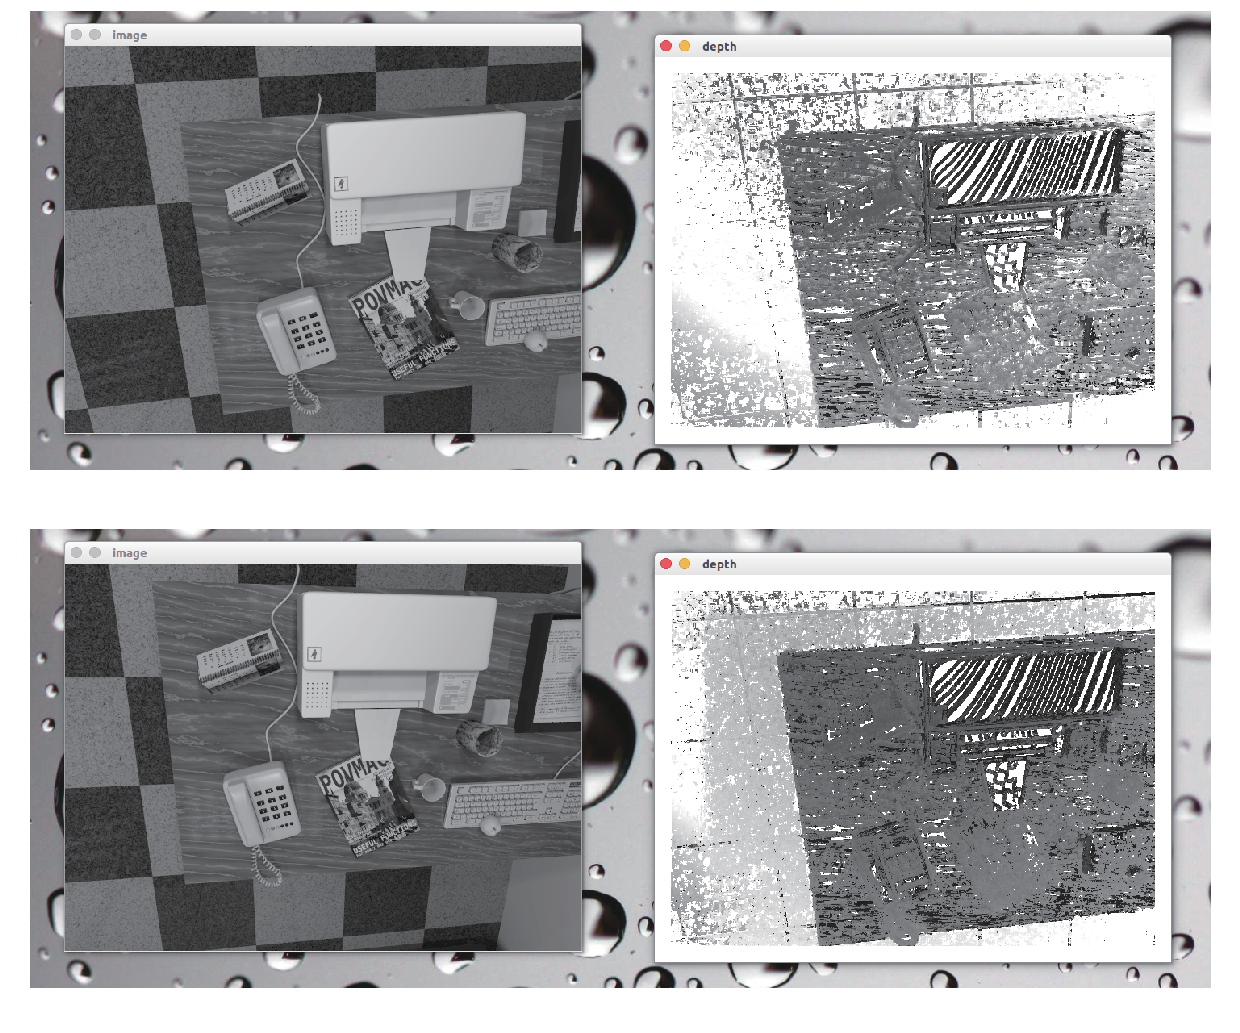
\includegraphics[width=.9\textwidth]{mapping/snapshot.pdf}
	\caption{演示程序运行时截图。两图分别是迭代10次和30次的结果。}
	\label{fig:snapshot}
\end{figure}

\clearpage
\section{实验分析与讨论}
上一节我们演示了移动单目相机的稠密建图,估计了参考帧的每个像素深度。我们的代码是相对简单直接的,没有使用许多的技巧(trick),因此出现了实际工程中常见的情形——简单的往往并不是最有效的。

由于真实数据的复杂性,能够在实际环境下工作的程序,往往需要周密的考虑和大量的工程技巧,这使得每种实际可行的代码都极其复杂——它们很难向初学者解释清楚,所以我们只好使用不那么有效,但相对易读易写的实现方式。我们当然可以提出若干种对演示程序加以改进的意见,不过这里并不打算把已经改好的(非常复杂的)程序直接呈现给读者。

下面我们对上一节实验的结果进行初步分析。我们将从计算机视觉和滤波器两个角度来分析演示实验的结果。

\subsection{像素梯度的问题}
对深度图像进行观察,我们会发现一件明显的事实。块匹配的正确与否,依赖于图像块是否具有区分度。显然,如果图像块仅是一片黑或者一片白,缺少有效的信息,那么在NCC计算中我们就很可能错误地将它与周围的某块像素给匹配起来。请读者观察演示程序中的打印机表面。由于它是均匀的白色,非常容易引起误匹配,因此打印机表面的深度信息多半是不正确的——示例程序的空间表面出现了明显不该有的条纹状深度估计,而根据我们的直观想象,打印机表面肯定是光滑的。

这里牵涉到了一个问题,该问题在直接法中我们已经见过一次。在进行块匹配(和NCC的计算)时,我们必须假设小块不变,然后将该小块与其他小块进行对比。这时,有\textbf{明显梯度}的小块将具有良好的区分度,不易引起误匹配。对于\textbf{梯度不明显的像素},由于在块匹配时没有区分性,所以我们将难以有效地估计其深度。反之,像素梯度比较明显的地方,我们得到的深度信息也相对准确,例如桌面上的杂志、电话等具有明显\textbf{纹理}的物体。因此,演示程序反映了立体视觉中一个非常常见的问题:\textbf{对物体纹理的依赖性}。该问题在双目视觉中也极其常见,体现了立体视觉的重建质量十分依赖于环境纹理。

我们的演示程序刻意使用了纹理较好的环境,例如,像棋盘格一般的地板,带有木纹的桌面,等等,因此能得到一个看似不错的结果。然而在实际中,像墙面、光滑物体表面等亮度均匀的地方将经常出现,影响我们对它的深度估计。从某种角度来说,该问题是\textbf{无法在现有的算法流程上加以改进并解决的}——如果我们依然只关心某个像素周围的邻域(小块)的话。

进一步讨论像素梯度问题,我们还会发现像素梯度和极线之间的联系。文章\cite{Engel2013}详细讨论过它们的关系,不过在我们的演示程序里也有直观的体现。

以\autoref{fig:epipolar-gradient}~为例,我们举两种比较极端的情况:像素梯度平行于极线方向,以及垂直于极线方向。先来看垂直的情况。在垂直的例子里,即使小块有明显梯度,但当我们沿着极线去做块匹配时,会发现匹配程度都是一样的,因此得不到有效的匹配。反之,在平行的例子里,我们能够精确地确定匹配度最高点出现在何处。而实际当中,梯度与极线的情况很可能介于二者之间:既不是完全垂直亦不是完全平行。这时,我们说,当像素梯度与极线夹角较大时,极线匹配的不确定性大;而当夹角较小时,匹配的不确定性变小。而在演示程序中,我们统一地把这些情况都当成一个像素的误差,实际是不够精细的。考虑到极线与像素梯度的关系后,应该使用更精确的不确定性模型。具体的调整和改进留作习题。

\begin{figure}[!htp]
	\centering
	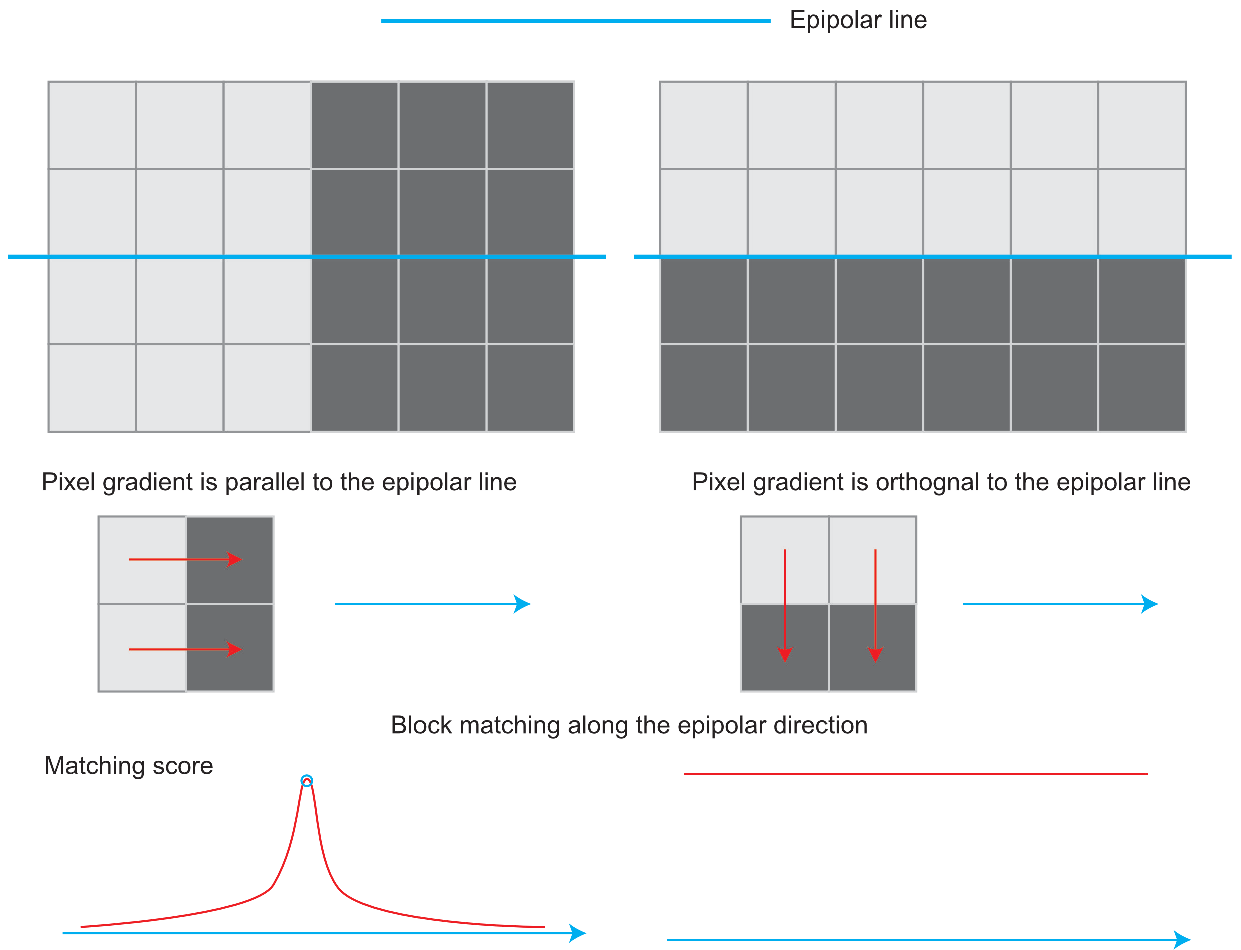
\includegraphics[width=1.0\textwidth]{mapping/epipolar-gradient.pdf}
	\caption{像素梯度与极线之关系示意图。}
	\label{fig:epipolar-gradient}
\end{figure}

\subsection{逆深度}
从另一个角度看,我们不妨问:把像素深度假设成高斯分布是否合适呢?这里关系到一个参数化的问题(Parameterization)。

\clearpage
在前面的内容中,我们经常用一个点的世界坐标$x,y,z$三个量来描述它,这是一种参数化形式。我们认为$x,y,z$三个量都是随机的,它们服从(三维的)高斯分布。然而,本讲使用了图像坐标$u,v$和深度值$d$来描述某个空间点(即稠密建图)。我们认为$u,v$不动,而$d$服从(一维的)高斯分布,这是另一种参数化形式。那么我们要问:这两种参数化形式有什么不同吗?我们是否也能假设$u,v$服从高斯分布,从而形成另一种参数化形式呢?

不同的参数化形式,实际都描述了同一个量,也就是某个三维空间点。考虑到当我们在相机看到某个点时,它的图像坐标$u,v$是比较确定的\footnote{$u,v$的不确定性取决于图像的分辨率。},而深度值$d$则是非常不确定的。此时,若用世界坐标$x,y,z$描述这个点,那么根据相机当前的位姿,$x,y,z$三个量之间可能存在明显的相关性。反映在协方差矩阵中,表现为非对角元素不为零。而如果用$u,v,d$参数化一个点,那么它的$u,v$和$d$至少是近似独立的,甚至我们还能认为$u,v$也是独立的——从而它的协方差矩阵近似为对角阵,更为简洁。

逆深度(Inverse depth)是近年来SLAM研究中出现的一种广泛使用的参数化技巧\textsuperscript{\cite{Montiel2006, Civera2008}}。在演示程序中,我们假设深度值满足高斯分布:$d \sim N(\mu, \sigma^2)$。然而这样做合不合理呢?深度真的近似于一个高斯分布吗?仔细想想,深度的正态分布确实存在一些问题:

\begin{enumerate}
	\item 我们实际想表达的是:这个场景深度大概是5\textasciitilde10米,可能有一些更远的点,但近处肯定不会小于相机焦距(或认为深度不会小于0)。这个分布并不是像高斯分布那样,形成一个对称的形状。它的尾部可能稍长,而负数区域则为零。
	\item 在一些室外应用中,可能存在距离非常远,乃至无穷远处的点。我们的初始值中难以涵盖这些点,并且用高斯分布描述它们会有一些数值计算上的困难。
\end{enumerate}

于是,逆深度应运而生。人们在仿真中发现,假设深度的倒数,也就是\textbf{逆深度},为高斯分布是比较有效的\textsuperscript{\cite{Civera2008}}。随后,在实际应用中,逆深度也具有更好的数值稳定性,从而逐渐成为一种通用的技巧,存在于现有SLAM方案中的标准做法中\textsuperscript{\cite{Forster2014, Engel2014, Mur-Artal2015}}。

把演示程序从正深度改成逆深度亦不复杂。只要在前面出现深度的推导中,将$d$改成逆深度$d^{-1}$即可。我们亦把这个改动留作习题,交给读者完成。

\subsection{图像间的变换}
在块匹配之前,做一次图像到图像间的变换亦是一种常见的预处理方式。这是因为,我们假设了图像小块在相机运动时保持不变,而这个假设在相机平移时(示例数据集基本都是这样的例子)能够保持成立,但当相机发生明显的旋转时,就难以继续保持了。特别地,当相机绕光心旋转时,一块下黑上白的图像可能会变成一个上黑下白的图像块,导致相关性直接变成了负数(尽管仍然是同样一个块)。

为了防止这种情况的出现,我们通常需要在块匹配之前,把参考帧与当前帧之间的运动考虑进来。根据相机模型,参考帧上的一个像素$\bm{P}_R$与真实的三维点世界坐标$\bm{P}_W$有以下关系:
\begin{equation}
d_R {\bm{P}_R} = \bm{K} \left( {{\bm{R}_{\mathrm{RW}}}{\bm{P}_W} + {\bm{t}_{\mathrm{RW}}}} \right).
\end{equation}

类似地,对于当前帧,亦有$\bm{P}_W$在它上边的投影,记作$\bm{P}_C$:
\begin{equation}
d_C {\bm{P}_C} = \bm{K} \left( {{\bm{R}_{\mathrm{CW}}}{\bm{P}_W} + {\bm{t}_{\mathrm{CW}}}} \right).
\end{equation}

代入并消去$\bm{P}_W$,即得两幅图像之间的像素关系:
\begin{equation}
d_C {\bm{P}_C} = d_R \bm{K} \bm{R}_{\mathrm{CW}} \bm{R}_{\mathrm{RW}}^\mathrm{T} \bm{K}^{-1} \bm{P}_R + \bm{K} \bm{t}_{\mathrm{CW}} - \bm{K} \bm{R}_{\mathrm{CW}} \bm{R}_{\mathrm{RW}}^\mathrm{T} \bm{K} \bm{t}_{\mathrm{RW}}.
\end{equation}

% 由于深度$d_C, d_R$未知,我们暂时把它们看作相同的,于是该式构成了一个从图像坐标到图像坐标的仿射变换。因此,我们可以把当前帧(或参考帧)进行变换后,再进行块匹配,以期获得对旋转更好的效果。存在一些稍有不同的仿射变换做法,例如\cite{Klein2007}中求解图像坐标的相对导数来计算仿射,也是可行的。
当知道$d_R, \bm{P}_R$时,可以计算出$\bm{P}_C$的投影位置。此时,再给$\bm{P}_R$两个分量各一个增量$\mathrm{d}u, \mathrm{d}v$,就可以求得$\bm{P}_C$的增量$\mathrm{d}u_c, \mathrm{d}v_c$。通过这种方式,算出在局部范围内参考帧和当前帧图像坐标变换的一个线性关系构成仿射变换:
\begin{equation}
\left[ \begin{array}{l}
\mathrm{d}u_c\\
\mathrm{d}v_c
\end{array} \right] = \left[ {\begin{array}{*{20}{c}}
	{\frac{{\mathrm{d}u_c}}{{\mathrm{d}u}}}&{\frac{{\mathrm{d}u_c}}{{\mathrm{d}v}}}\\
	{\frac{{\mathrm{d}v_c}}{{\mathrm{d}u}}}&{\frac{{\mathrm{d}v_c}}{{\mathrm{d}v}}}
	\end{array}} \right]\left[ \begin{array}{l}
\mathrm{d}u\\
\mathrm{d}v
\end{array} \right]
\end{equation}

根据仿射变换矩阵,我们可以把当前帧(或参考帧)的像素进行变换后再进行块匹配,以期获得对旋转更好的效果。

\subsection{并行化:效率的问题}
在实验当中我们也看到,稠密深度图的估计非常费时,这是因为我们要估计的点从原先的数百个特征点一下子变成了几十万个像素点,即使现在主流的CPU也无法实时地计算那样庞大的数量。不过,该问题亦有另一个性质:这几十万个像素点的深度估计是彼此无关的!这使并行化有了用武之地。

在示例程序中,我们在一个二重循环里遍历了所有像素,并逐个对它们进行极线搜索。当我们使用CPU时,这个过程是串行进行的:必须是上一个像素计算完毕后,再计算下一个像素。然而实际上,下一个像素完全没有必要等待上一个像素的计算结束,因为它们之间并没有明显的联系,所以我们可以用多个线程,分别计算每个像素,然后将结果统一起来。理论上,如果我们有30万个线程,那么该问题的计算时间和计算一个像素是一样的。

GPU的并行计算架构非常适合这样的问题,因此,在单双和双目的稠密重建中,经常看到利用GPU进行并行加速的方式。当然,本书不准备涉及GPU编程,所以我们在这里仅指出利用GPU加速的可能性,具体实践留给读者作为验证。根据一些类似的工作,利用GPU的稠密深度估计是可以在主流GPU上实时化的。

\subsection{其他的改进}
事实上,我们还能提出许多对本例程进行改进的方案,例如:

\begin{enumerate}
	\item 现在各像素完全是独立计算的,可能存在这个像素深度很小,边上一个又很大的情况。我们可以假设深度图中相邻的深度变化不会太大,从而给深度估计加上了空间正则项。这种做法会使得到的深度图更加平滑。
	\item 我们没有显式地处理外点(Outlier)的情况。事实上,由于遮挡、光照、运动模糊等各种因素的影响,不可能对每个像素都能保持成功匹配。而演示程序的做法中,只要NCC大于一定值,就认为出现了成功的匹配,没有考虑到错误匹配的情况。
	
	\hspace{2em}处理错误匹配亦有若干种方式。例如,文献\cite{Vogiatzis2011}提出的均匀−高斯混合分布下的深度滤波器,显式地将内点与外点进行区别并进行概率建模,能够较好地处理外点数据。然而这种类型的滤波器理论较为复杂,本书不想过多涉及,读者可以阅读原始论文。
\end{enumerate}

从上面的讨论可以看出,存在着许多可能的改进方案。如果我们细致地改进每一步的做法,最后是有希望得到一个良好的稠密建图的方案的。然而,正如我们所讨论的,有一些问题\textbf{存在理论上的困难},例如对环境纹理的依赖,又如像素梯度与极线方向的关联(以及平行的情况)。这些问题\textbf{很难通过调整代码实现来解决}。所以,直到目前为止,尽管双目和移动单目能够建立稠密的地图,我们通常认为它们过于依赖于环境纹理和光照,不够可靠。

\section{RGB-D 稠密建图}
除了使用单目和双目进行稠密重建之外,在适用范围内,RGB-D相机是一种更好的选择。在上一讲中详细讨论的深度估计问题,在RGB-D相机中可以完全通过传感器中硬件测量得到,无须消耗大量的计算资源来估计。并且,RGB-D的结构光或飞时原理,保证了深度数据对纹理的无关性。即使面对纯色的物体,只要它能够反射光,我们就能测量到它的深度。这亦是RGB-D传感器的一大优势。

利用RGB-D进行稠密建图是相对容易的。不过,根据地图形式不同,也存在着若干种不同的主流建图方式。最直观、最简单的方法,就是根据估算的相机位姿,将RGB-D数据转化为点云(Point Cloud),然后进行拼接,最后得到一个由离散的点组成的点云地图(Point Cloud Map)。在此基础上,如果我们对外观有进一步的要求,希望估计物体的表面,可以使用三角网格(Mesh)、面片(Surfel)进行建图。另一方面,如果希望知道地图的障碍物信息并在地图上导航,亦可通过体素(Voxel)建立占据网格地图(Occupancy Map)。

我们似乎引入了很多新概念。请读者不要着急,我们将慢慢地逐一加以介绍。对于部分适合进行实验的,我们亦会像往常一样,提供若干个演示程序。由于RGB-D建图牵涉到的理论知识并不很多,所以下面几节就直接以实践部分来介绍了。GPU建图超出了本书的范围,我们就简单讲解其原理,不做演示。

\subsection{实践:点云地图}
首先,我们来讲解最简单的点云地图。所谓点云,就是由一组离散的点表示的地图。最基本的点包含$x,y,z$三维坐标,也可以带有$r,g,b$的彩色信息。由于RGB-D相机提供了彩色图和深度图,很容易根据相机内参来计算RGB-D点云。如果通过某种手段,得到了相机的位姿,那么只要直接把点云进行加和,就可以获得全局的点云。在本书的~\ref{sec:join-point-cloud}~节,曾给出了一个通过相机内外参拼接点云的例子。不过,那个例子主要是为了让读者理解相机的内外参,而在实际建图当中,我们还会对点云加一些滤波处理,以获得更好的视觉效果。在本程序中,我们主要使用两种滤波器:外点去除滤波器,以及降采样滤波器。示例程序的代码如下(由于部分代码与之前的相同,我们主要看改变的部分):

\begin{lstlisting}[language=c++,caption=slambook/ch13/dense\_RGBD/pointcloud\_mapping.cpp(片段)]
int main( int argc, char** argv )
{
	// 图像读取部分略
	// 定义点云使用的格式:这里用的是XYZRGB
	typedef pcl::PointXYZRGB PointT; 
	typedef pcl::PointCloud<PointT> PointCloud;
	
	// 新建一个点云
	PointCloud::Ptr pointCloud( new PointCloud ); 
	for ( int i=0; i<5; i++ )
	{
		PointCloud::Ptr current( new PointCloud );
		cout<<"转换图像中: "<<i+1<<endl; 
		cv::Mat color = colorImgs[i]; 
		cv::Mat depth = depthImgs[i];
		Eigen::Isometry3d T = poses[i];
		for ( int v=0; v<color.rows; v++ )
		for ( int u=0; u<color.cols; u++ )
		{
			unsigned int d = depth.ptr<unsigned short> ( v )[u]; // 深度值
			if ( d==0 ) continue; // 为 0 表示没有测量到
			if ( d >= 7000 ) continue; // 深度太大时不稳定,去掉
			Eigen::Vector3d point; 
			point[2] = double(d)/depthScale; 
			point[0] = (u-cx)*point[2]/fx;
			point[1] = (v-cy)*point[2]/fy; 
			Eigen::Vector3d pointWorld = T*point;
			
			PointT p ;
			p.x = pointWorld[0];
			p.y = pointWorld[1];
			p.z = pointWorld[2];
			p.b = color.data[ v*color.step+u*color.channels() ];
			p.g = color.data[ v*color.step+u*color.channels()+1 ];
			p.r = color.data[ v*color.step+u*color.channels()+2 ];
			current->points.push_back( p );
		}
		// depth filter and statistical removal 
		PointCloud::Ptr tmp ( new PointCloud );
		pcl::StatisticalOutlierRemoval<PointT> statistical_filter;
		statistical_filter.setMeanK(50);
		statistical_filter.setStddevMulThresh(1.0);
		statistical_filter.setInputCloud(current);
		statistical_filter.filter( *tmp );
		(*pointCloud) += *tmp;
	}
	
	pointCloud->is_dense = false;
	cout<<"点云共有"<<pointCloud->size()<<"个点."<<endl;
	
	// voxel filter 
	pcl::VoxelGrid<PointT> voxel_filter; 
	voxel_filter.setLeafSize( 0.01, 0.01, 0.01 );       // resolution 
	PointCloud::Ptr tmp ( new PointCloud );
	voxel_filter.setInputCloud( pointCloud );
	voxel_filter.filter( *tmp );
	tmp->swap( *pointCloud );
	
	cout<<"滤波之后,点云共有"<<pointCloud->size()<<"个点."<<endl;
	
	pcl::io::savePCDFileBinary("map.pcd", *pointCloud );
	return 0;
}
\end{lstlisting}

\clearpage
我们的思路没有太大变化,主要不同之处在于:

\begin{enumerate}
	\item 在生成每帧点云时,去掉深度值太大或无效的点。这主要是考虑到Kinect的有效量程,超过量程之后的深度值会有较大误差。
	\item 利用统计滤波器方法去除孤立点。该滤波器统计每个点与距离它最近的$N$个点的距离值的分布,去除距离均值过大的点。这样,我们保留了那些“粘在一起”的点,去掉了孤立的噪声点。
	\item 最后,利用体素滤波器(Voxel Filter)进行降采样。由于多个视角存在视野重叠,在重叠区域会存在大量的位置十分相近的点。这会白白占用许多内存空间。体素滤波保证了在某个一定大小的立方体(或称体素)内仅有一个点,相当于对三维空间进行了降采样,从而可节省很多存储空间。
\end{enumerate}

\autoref{fig:pcd-filter}~显示了滤波前后的对比图。左侧是第5讲程序生成的点云地图,而右侧是经过滤波后的点云地图。观察白色框中部分,可以看到在滤波前存在着由噪声产生的许多孤立的点。经过统计外点去除之后,我们消去了这些噪声,使得整个地图变得更干净。另一方面,我们在体素滤波器中,把分辨率调至0.01,表示每立方厘米有一个点。这是一个比较高的分辨率,所以在截图中我们感觉不出地图的差异,然而从程序输出中可以看到点数明显减少了许多(从90万个点减到了44万个点,去除了一半左右)。

\begin{figure}[!ht]
	\centering
	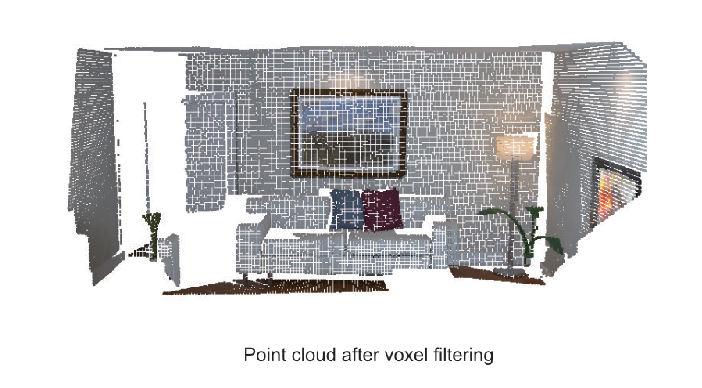
\includegraphics[width=1.0\textwidth]{mapping/pcd-filter.pdf}
	\caption{滤波前后的对比图(你可能需要放大才能看清,或者自己在电脑上尝试一下)。}
	\label{fig:pcd-filter}
\end{figure}

点云地图为我们提供了比较基本的可视化地图,让我们能够大致了解环境的样子。它以三维方式存储,使得我们能够快速地浏览场景的各个角落,乃至在场景中进行漫游。点云的一大优势是可以直接由RGB-D图像高效地生成,不需要额外处理。它的滤波操作也非常直观,且处理效率尚能接受。

不过,使用点云表达地图仍然是十分初级的,我们不妨按照之前提的对地图的需求,看看点云地图是否能满足。
\enlargethispage{-3pt}
\begin{enumerate}
	\item 定位需求:取决于前端视觉里程计的处理方式。如果是基于特征点的视觉里程计,由于点云中没有存储特征点信息,所以无法用于基于特征点的定位方法。如果前端是点云的ICP,那么可以考虑将局部点云对全局点云进行ICP以估计位姿。然而,这要求全局点云具有较好的精度。在我们这种处理点云的方式中,并没有对点云本身进行优化,所以是不够的。
	\item 导航与避障的需求:无法直接用于导航和避障。纯粹的点云无法表示“是否有障碍物”的信息,我们也无法在点云中做“任意空间点是否被占据”这样的查询,而这是导航和避障的基本需要。不过,可以在点云基础上进行加工,得到更适合导航与避障的地图形式。
	\item 可视化和交互:具有基本的可视化与交互能力。我们能够看到场景的外观,也能在场景里漫游。从可视化角度来说,由于点云只含有离散的点,而没有物体表面信息(例如法线),所以不太符合人们的可视化习惯。例如,点云地图的物体从正面看和背面看是一样的,而且还能透过物体看到它背后的东西:这些都不符合我们日常的经验,因为我们没有物体表面的信息。
\end{enumerate}

综上所述,我们说点云地图是“基础的”或“初级的”,是指它更接近于传感器读取的原始数据。它具有一些基本的功能,但通常用于调试和基本的显示,不便直接用于应用程序。如果我们希望地图有更高级的功能,点云地图是一个不错的出发点。例如,针对导航功能,我们可以从点云出发,构建占据网格地图(Occupancy Grid),以供导航算法查询某点是否可以通过。再如,SfM中常用的泊松重建\textsuperscript{\cite{Kazhdan2006}}方法,就能通过基本的点云重建物体网格地图,得到物体的表面信息。除泊松重建外,Surfel亦是一种表达物体表面的方式,以面元作为地图的基本单位,能够建立漂亮的可视化地图\textsuperscript{\cite{Stuckler2014}}。

\autoref{fig:poisson-surfel}~显示了泊松重建和Surfel的一个样例,可以看到它们的视觉效果明显优于纯粹点云建图,而它们都可以通过点云进行构建。大部分由点云转换得到的地图形式都在PCL库中提供,感兴趣的读者可以进一步探索PCL库内容。而本书作为入门材料,就不详尽地介绍每一种地图形式了。

\begin{figure}[!htp]
	\centering
	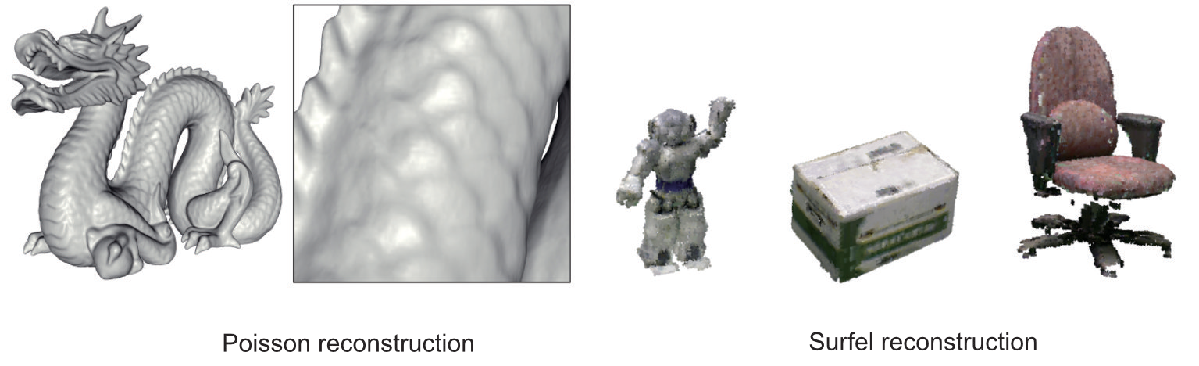
\includegraphics[width=1.0\textwidth]{mapping/poisson-surfel.pdf}
	\caption{泊松重建与Surfel的示意图。}
	\label{fig:poisson-surfel}
\end{figure}

\subsection{八叉树地图}
下面介绍一种在导航中比较常用的,本身有较好的压缩性能的地图形式:\textbf{八叉树地图}。

在点云地图中,我们虽然有了三维结构,也进行了体素滤波以调整分辨率,但是点云有几个明显的缺陷:

\begin{itemize}
	\item 点云地图通常规模很大,所以pcd文件也会很大。一幅$640$像素$\times480$像素的图像,会产生30万个空间点,需要大量的存储空间。即使经过一些滤波后,pcd文件也是很大的。而且讨厌之处在于,它的“大”并不是必需的。点云地图提供了很多不必要的细节。对于地毯上的褶皱、阴暗处的影子,我们并不特别关心这些东西。把它们放在地图里是在浪费空间。由于这些空间的占用,除非我们降低分辨率,否则在有限的内存中,无法建模较大的环境。然而降低分辨率会导致地图质量下降。有没有什么方式对地图进行压缩存储,舍弃一些重复的信息呢?
	\item 点云地图无法处理运动物体。因为我们的做法里只有“添加点”,而没有“当点消失时把它移除”的做法。而在实际环境中,运动物体的普遍存在,使得点云地图变得不够实用。
\end{itemize}

而我们接来下要介绍的,就是一种灵活的、压缩的、又能随时更新的地图形式:八叉树(Octo-map)\textsuperscript{\cite{Hornung2013}}。

我们知道,把三维空间建模为许多个小方块(或体素)是一种常见的做法。如果我们把一个小方块的每个面平均切成两片,那么这个小方块就会变成同样大小的八个小方块。这个步骤可以不断地重复,直到最后的方块大小达到建模的最高精度。在这个过程中,把“将一个小方块分成同样大小的八个”这件事,看成“从一个节点展开成八个子节点”,那么,整个从最大空间细分到最小空间的过程,就是一棵八叉树(Octo-tree)。

如\autoref{fig:octomap}~所示,左侧显示了一个大立方体不断地均匀分成八块,直到变成最小的方块为止。于是,整个大方块可以看成是根节点,而最小的块可以看作是“叶子节点”。于是,在八叉树中,当我们由下一层节点往上走一层时,地图的体积就能扩大为原来的八倍。我们不妨做一点简单的计算:如果叶子节点的方块大小为1 cm$^3$,那么当我们限制八叉树为10层时,总共能建模的体积大约为$8^{10}\text{cm}^3 = 1,073\text{m}^3$,这足够建模一间屋子。由于体积与深度呈指数关系,所以当我们用更大的深度时,建模的体积会增长得非常快。

\begin{figure}[!ht]
	\centering
	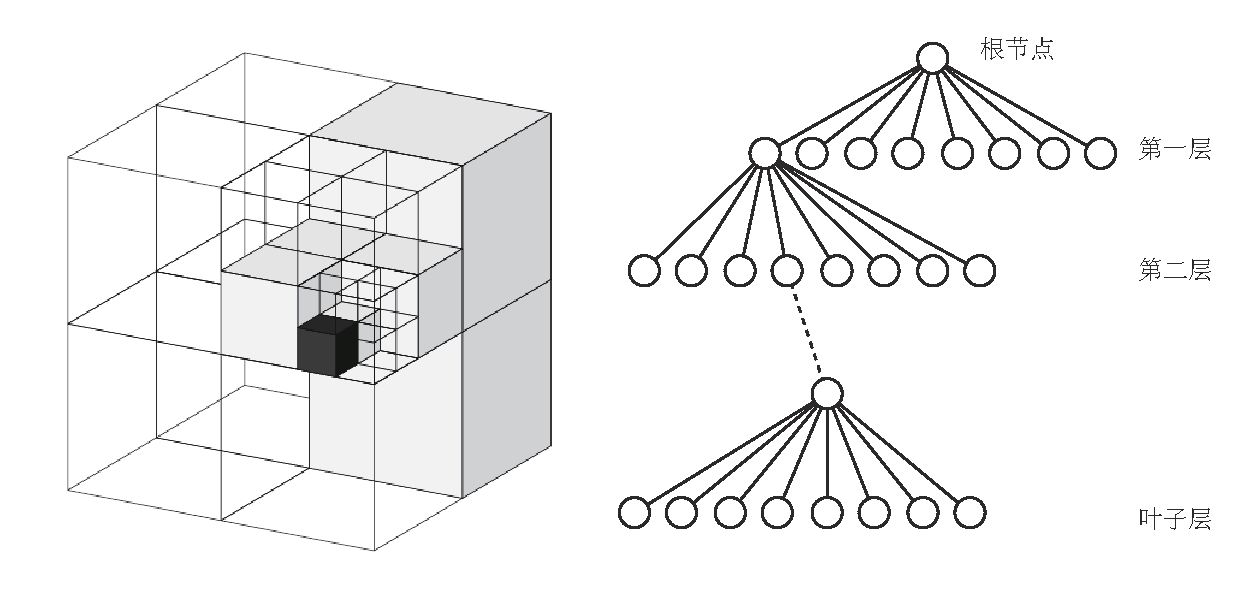
\includegraphics[width=1.0\textwidth]{mapping/octomap.pdf}
	\caption{八叉树示意图。}
	\label{fig:octomap}
\end{figure}

读者可能会疑惑,在点云的体素滤波器中,我们不是也限制了一个体素中只有一个点吗?为何我们说点云占空间,而八叉树比较节省空间呢?这是因为,在八叉树中,我们在节点中存储它是否被占据的信息。然而,不同之处在于,当某个方块的所有子节点都被占据或都不被占据时,就\textbf{没必要展开这个节点}。例如,一开始地图为空白时,我们就只需一个根节点,而不需要完整的树。当向地图中添加信息时,由于实际的物体经常连在一起,空白的地方也会常常连在一起,所以大多数八叉树节点都无须展开到叶子层面。所以说,八叉树比点云节省大量的存储空间。

\newpage
前面说八叉树的节点存储了它是否被占据的信息。从点云层面来讲,我们自然可以用0表示空白,1表示被占据。这种0−1的表示可以用一个比特来存储,节省空间,不过显得有些过于简单了。由于噪声的影响,我们可能会看到某个点一会儿为0,一会儿为1;或者大部分时刻为0,小部分时刻为1;或者除了“是”“否”两种情况之外,还有一个“未知”的状态。能否更精细地描述这件事呢?我们会选择用\textbf{概率}形式表达某节点是否被占据的事情。比如,用一个浮点数$x \in [0,1]$来表达。这个$x$一开始取0.5。如果不断观测到它被占据,那么让这个值不断增加;反之,如果不断观测到它是空白,那就让它不断减小即可。

通过这种方式,我们动态地建模了地图中的障碍物信息。不过,现在的方式有一点小问题:如果让$x$不断增加或减小,它可能跑到$[0,1]$区间之外,带来处理上的不便。所以我们不是直接用概率来描述某节点被占据,而是用概率对数值(Log-odds)来描述。设$y \in \mathbb{R}$为概率对数值,$x$为0\textasciitilde1的概率,那么它们之间的变换由logit变换描述:
\begin{equation}
y = \mathrm{logit}(x) = \log \left( \frac{x}{1-x} \right).
\end{equation}

其反变换为
\begin{equation}
x = \mathrm{logit}^{-1}(y) = \frac{\exp(y)}{\exp(y)+1}.
\end{equation}

\enlargethispage{4pt}
可以看到,当$y$从$-\infty$变到$+\infty$时,$x$相应地从0变到了1。而当$y$取0时,$x$取到0.5。因此,我们不妨存储$y$来表达节点是否被占据。当不断观测到“占据”时,让$y$增加一个值;否则就让$y$减小一个值。当查询概率时,再用逆logit变换,将$y$转换至概率即可。用数学形式来说,设某节点为$n$,观测数据为$z$。那么从开始到$t$时刻某节点的概率对数值为$L(n|z_{1:t})$,$t+1$时刻为
\clearpage
\begin{equation}
L(n|z_{1:t+1}) = L(n|z_{1:t-1}) + L(n|z_{t}).
\end{equation}

如果写成概率形式而不是概率对数形式,就会有一点复杂:
\begin{equation}
P(n|z_{1:T}) =  \left[ 1+ \frac{1-P(n|z_T)}{P(n|z_T)} \frac{1-P(n|z_{1:T-1})}{P(n|z_{1:T-1})} \frac{P(n)}{1-P(n)} \right]^{-1}.
\end{equation}

有了对数概率,我们就可以根据RGB-D数据更新整个八叉树地图了。假设我们在RGB-D图像中观测到某个像素带有深度$d$,这说明了一件事:我们\textbf{在深度值对应的空间点上观察到了一个占据数据,并且,从相机光心出发到这个点的线段上,应该是没有物体的}(否则会被遮挡)。利用这个信息,可以很好地对八叉树地图进行更新,并且能处理运动的结构。

\subsection{实践:八叉树地图}
下面通过程序演示一下octomap的建图过程。首先,请读者安装octomap库:\url{https://github.com/OctoMap/octomap}。Octomap库主要包含octomap地图与octovis(一个可视化程序),二者都是cmake工程。其主要依赖doxygen,可通过如下命令安装:
\begin{lstlisting}
sudo apt-get install doxygen 
\end{lstlisting}

我们直接来演示如何通过前面的5张图像生成八叉树地图,然后将它画出来。

\begin{lstlisting}[language=c++,caption=slambook/ch13/dense\_RGBD/octomap\_mapping.cpp(片段)]
#include <iostream>
#include <fstream>
using namespace std;

#include <opencv2/core/core.hpp>
#include <opencv2/highgui/highgui.hpp>

#include <octomap/octomap.h>    // for octomap 

#include <Eigen/Geometry> 
#include <boost/format.hpp>  // for formating strings

int main( int argc, char** argv )
{
	// 图像和位姿读取部分略
	cout<<"正在将图像转换为 Octomap ..."<<endl;
	
	// octomap tree 
	octomap::OcTree tree( 0.05 ); // 参数为分辨率
	
	for ( int i=0; i<5; i++ )
	{
		cout<<"转换图像中: "<<i+1<<endl; 
		cv::Mat color = colorImgs[i]; 
		cv::Mat depth = depthImgs[i];
		Eigen::Isometry3d T = poses[i];
		
		octomap::Pointcloud cloud;  // the point cloud in octomap 
		
		for ( int v=0; v<color.rows; v++ )
			for ( int u=0; u<color.cols; u++ )
			{
				unsigned int d = depth.ptr<unsigned short> ( v )[u]; // 深度值
				if ( d==0 ) continue; // 为0表示没有测量到
				if ( d >= 7000 ) continue; // 深度太大时不稳定,去掉
				Eigen::Vector3d point; 
				point[2] = double(d)/depthScale; 
				point[0] = (u-cx)*point[2]/fx;
				point[1] = (v-cy)*point[2]/fy; 
				Eigen::Vector3d pointWorld = T*point;
				// 将世界坐标系的点放入点云
				cloud.push_back( pointWorld[0], pointWorld[1], pointWorld[2] ); 
			}
	
		// 将点云存入八叉树地图,给定原点,这样可以计算投射线
		tree.insertPointCloud( cloud, octomap::point3d( T(0,3), T(1,3), T(2,3) ) );     
	}
	
	// 更新中间节点的占据信息并写入磁盘
	tree.updateInnerOccupancy();
	cout<<"saving octomap ... "<<endl;
	tree.writeBinary( "octomap.bt" );
	return 0;
}
\end{lstlisting}

我们使用了octomap::OcTree来构建整张地图。实际上,octomap提供了许多种八叉树:有带地图的,有带占据信息的,你也可以自己定义每个节点需要携带哪些变量。简单起见,我们使用了不带颜色信息的、最基本的八叉树地图。

Ocotmap内部提供了一个点云结构。它比PCL的点云稍微简单一些,只携带点的空间位置信息。我们根据RGB-D图像和相机位姿信息,先将点的坐标转至世界坐标,然后放入octomap的点云,最后交给八叉树地图。之后,octomap会根据之前介绍的投影信息,更新内部的占据概率,最后保存成压缩后的八叉树地图。我们把生成的地图存成octomap.bt文件。在之前编译octovis时,我们实际上安装了一个可视化程序,即octovis。现在,调用它打开地图文件,就能看到地图的实际样子了。

\autoref{fig:octomap-result}~显示了我们构建的地图结果。由于我们没有在地图中加入颜色信息,所以一开始打开地图时将是灰色的,按“1”键可以根据高度信息进行染色。读者可以熟悉一下octovis的操作界面,包括地图的查看、旋转、缩放等。

\begin{figure}[!htp]
	\centering
	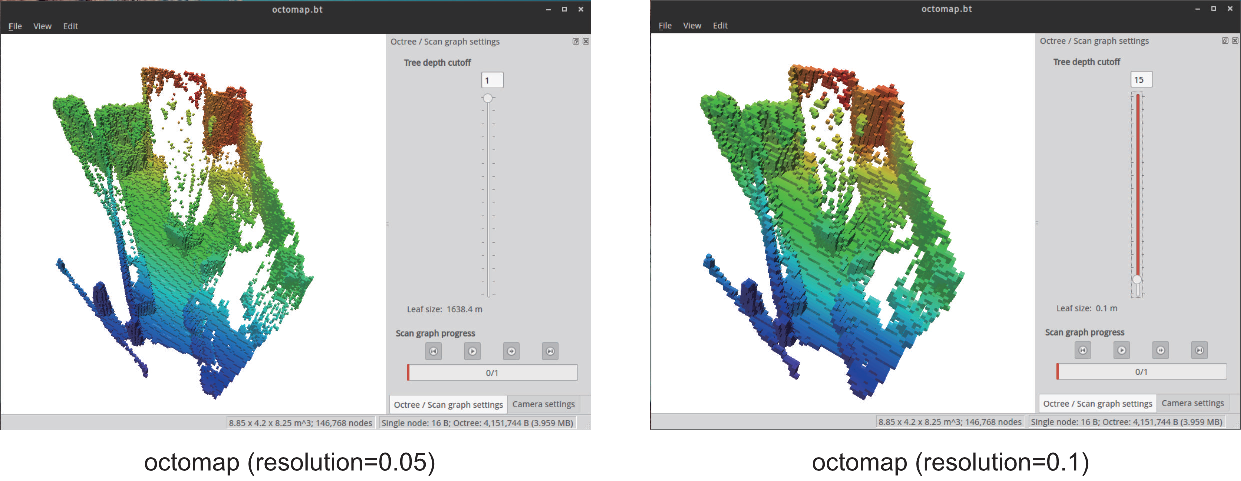
\includegraphics[width=1.0\textwidth]{mapping/octomap-result.pdf}
	\caption{八叉树地图在不同分辨率下的显示结果。}
	\label{fig:octomap-result}
\end{figure}

在右侧有八叉树的深度限制条,这里可以调节地图的分辨率。由于我们构造时使用的默认深度是16层,所以这里显示16层即最高分辨率,也就是每个小块的边长为0.05米。当我们将深度减少一层时,八叉树的叶子节点往上提一层,每个小块的边长就增加一倍,变成0.1米。可以看到,我们能够很容易地调节地图分辨率以适应不同的场合。

Octomap还有一些可以探索的地方,例如,我们可以方便地查询任意点的占据概率,以此设计在地图中进行导航的方法\textsuperscript{\cite{Burri2015}}。读者亦可比较点云地图与八叉树地图的文件大小。上一节生成的点云地图的磁盘文件大约为6.9MB,而octomap只有56KB,连点云地图的百分之一都不到,可以有效地建模较大的场景。

\section{\textsuperscript{\ttfamily *} TSDF地图和Fusion系列}

在本讲的最后,我们介绍一个与SLAM非常相似但又有稍许不同的研究方向:实时三维重建。本节内容牵涉到GPU编程,并未提供参考例子,所以作为可选的阅读材料。

在前面的地图模型中,\textbf{以定位为主体}。地图的拼接是作为后续加工步骤放在SLAM框架中的。这种框架成为主流的原因是,定位算法可以满足实时性的需求,而地图的加工可以在关键帧处进行处理,无须实时响应。定位通常是轻量级的,特别是当使用稀疏特征或稀疏直接法时;相应地,地图的表达与存储则是重量级的。它们的规模和计算需求较大,不利于实时处理。特别是稠密地图,往往只能在关键帧层面进行计算。

但是,现有做法中,我们并没有对稠密地图进行优化。比如,当两幅图像都观察到同一把椅子时,我们只根据两幅图像的位姿把两处的点云进行叠加,生成了地图。由于位姿估计通常是带有误差的,这种直接拼接往往不够准确,比如同一把椅子的点云无法完美地叠加在一起。这时候,地图中会出现这把椅子的两个重影——这种现象有时候被形象地称为“鬼影”。

这种现象显然不是我们想要的,我们希望重建结果是光滑的、完整的,符合我们对地图的认识的。在这种思想下,出现了一种以“建图”为主体,而定位居于次要地位的做法,也就是本节要介绍的实时三维重建。由于三维重建把重建准确地图作为主要目标,所以基本都需要利用GPU进行加速,甚至需要非常高级的GPU或多个GPU进行并行加速,通常需要较重的计算设备。与之相反,SLAM是朝轻量级、小型化方向发展,有些方案甚至放弃了建图和回环检测部分,只保留了视觉里程计。而实时重建则正在朝大规模、大型动态场景的重建方向发展。

自从RGB-D传感器出现以来,利用RGB-D图像进行实时重建形成了一个重要的发展方向,陆续产生了Kinect Fusion\textsuperscript{\cite{Newcombe2011}}、Dynamic Fusion\textsuperscript{\cite{Newcombe2015}}、Elastic Fusion\textsuperscript{\cite{Whelan2015}}、Fusion4D\textsuperscript{\cite{Dou2016}}、Volume Deform\textsuperscript{\cite{Innmann2016}}等成果。其中,Kinect Fusion完成了基本的模型重建,但仅限于小型场景;后续的工作则是将它向大型的、运动的,甚至变形场景下拓展。我们把它们看成实时重建一个大类的工作,但由于种类繁多,不可能详细讨论每一种的工作原理。\autoref{fig:fusions}~展示了一部分重建结果,可以看到这些建模结果非常精细,比单纯拼接点云要细腻很多。

\begin{figure}[!htp]
	\centering
	\includegraphics[width=0.9\textwidth]{mapping/fusions.pdf}
	\caption{各种实时三维重建的模型。(a)Kinect Fusion;(b)Dynamic Fusion;(c)Volume Deform;(d)Fusion4D;(e)Elastic Fusion。}
	\label{fig:fusions}
\end{figure}

我们就以经典的TSDF地图为代表进行介绍。TSDF是Truncated Signed Distance Function的缩写,不妨译作\textbf{截断符号距离函数}。虽然把“函数”称为“地图”似乎不太妥当,然而在没有更好的翻译之前,我们还是暂时称它为TSDF地图、TSDF重建等,只要不产生理解上的偏差即可。

与八叉树相似,TSDF地图也是一种网格式(或者说,方块式)的地图,如\autoref{fig:tsdf}所示。先选定要建模的三维空间,比如$3\times3\times3 \text{m}^3$那么大,按照一定分辨率将这个空间分成许多小块,存储每个小块内部的信息。不同的是,TSDF地图整个存储在显存而不是内存中。利用GPU的并行特性,我们可以并行地对每个体素进行计算和更新,而不像CPU遍历内存区域那样不得不串行。

\begin{figure}[!t]
	\centering
	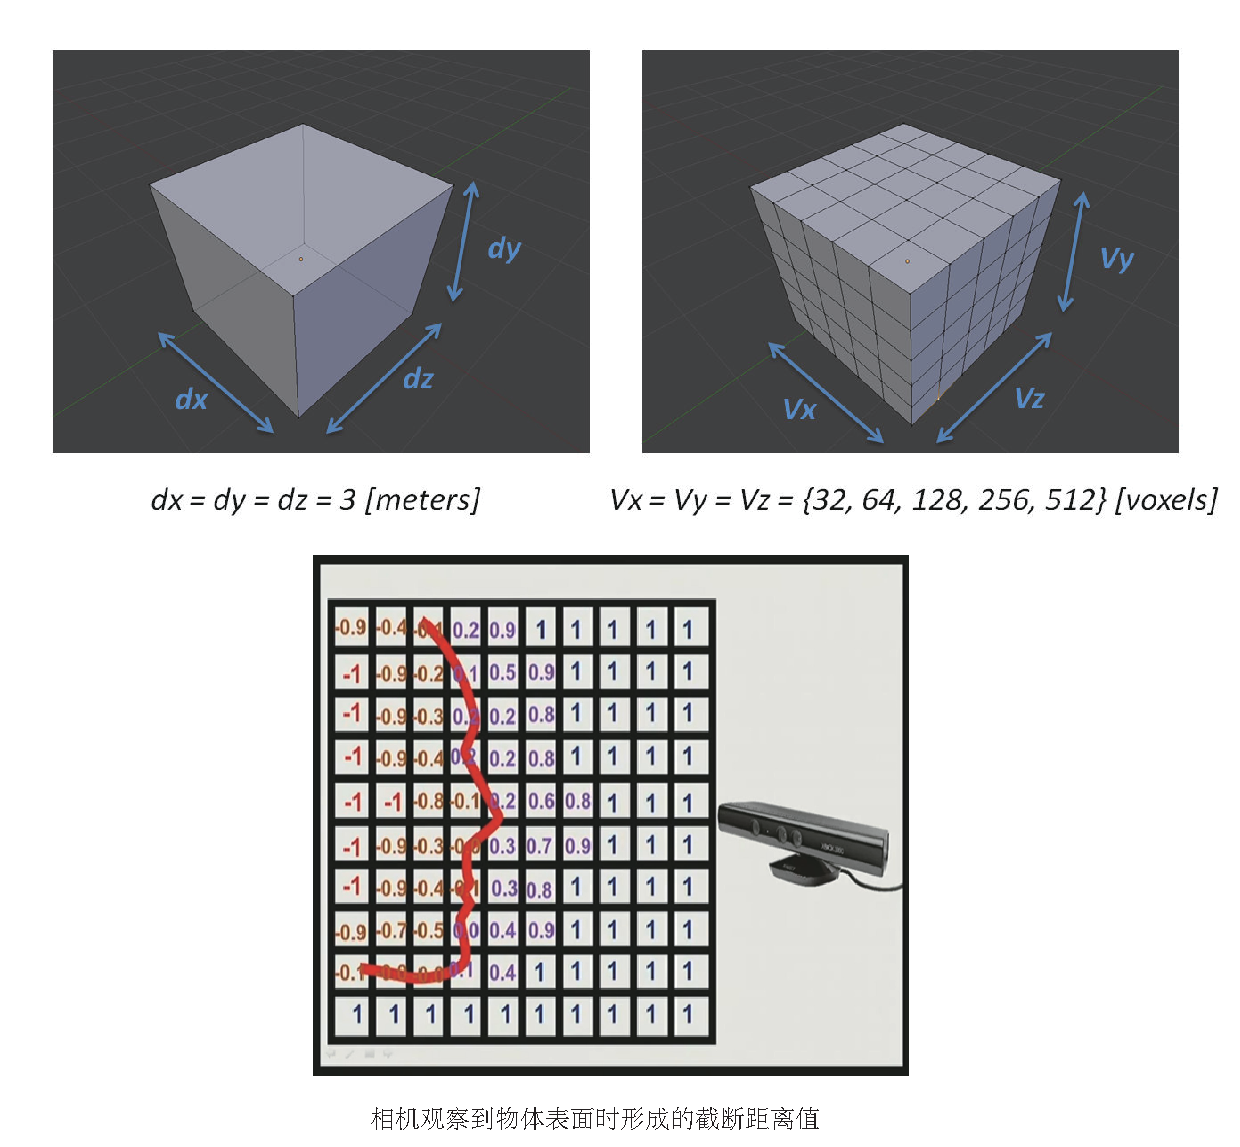
\includegraphics[width=1.0\textwidth]{mapping/tsdf.pdf}
	\caption{TSDF示意图。}
	\label{fig:tsdf}
\end{figure}

每个TSDF体素内,存储了该小块与距其最近的物体表面的距离。如果小块在该物体表面的前方,它就有一个正的值;反之,如果该小块位于表面之后,那么就为负值。由于物体表面通常是很薄的一层,所以就把值太大的和太小的都取成$1$和$-1$,这样就得到了截断之后的距离,也就是所谓的TSDF。那么按照定义,TSDF为0的地方就是表面本身——或者,由于数值误差的存在,TSDF由负号变成正号的地方就是表面本身。在\autoref{fig:tsdf}~的下部,我们看到一个类似于人脸的表面出现在了TSDF改变符号的地方。

\newpage
\enlargethispage{4pt}
TSDF亦有“定位”与“建图”两个问题,与SLAM非常相似,不过具体的形式与本书前面几讲介绍的稍有不同。在这里,定位问题主要指如何把当前的RGB-D图像与GPU中的TSDF地图进行比较,估计相机位姿。而建图问题就是如何根据估计的相机位姿,对TSDF地图进行更新。传统做法中,我们还会对RGB-D图像进行一次双边贝叶斯滤波,以去除深度图中的噪声。

TSDF的定位类似于前面介绍的ICP,不过由于GPU的并行化,我们可以对整张深度图和TSDF地图进行ICP计算,而不必像传统视觉里程计那样必须先计算特征点。同时,由于TSDF没有颜色信息,意味着我们可以\textbf{只使用深度图},不使用彩色图,就完成位姿估计,这在一定程度上摆脱了视觉里程计算法对光照和纹理的依赖性,使得RGB-D重建更加稳健\footnote{不过话说回来,对深度图就更加依赖了。}。另一方面,建图部分亦是一种并行地对TSDF中的数值进行更新的过程,使得所估计的表面更加平滑可靠。由于我们并不过多介绍GPU相关的内容,所以具体的方法就不展开细说了,请感兴趣的读者参阅相关文献。

\section{小结}
本讲介绍了一些常见的地图类型,尤其是稠密地图形式。我们看到根据单目或双目可以构建稠密地图,而RGB-D地图则往往更加容易、稳定一些。本讲的地图偏重于度量地图,而拓扑地图形式由于和SLAM研究差别比较大,所以没有详细地展开探讨。

\section*{习题}
\begin{enumerate}
	\item 推导式(13.6)。
	\item 把本讲的稠密深度估计改成半稠密,你可以先把梯度明显的地方筛选出来。
	\item[\optional] 把本讲演示的单目稠密重建代码从正深度改成逆深度,并添加仿射变换。你的实验效果是否有改进?
	\item 你能论证如何在八叉树中进行导航或路径规划吗?
	\item 研究文献\cite{Newcombe2011},探讨TSDF地图是如何进行位姿估计和更新的。它和我们之前讲过的定位建图算法有何异同?
	\item[\optional] 研究均匀−高斯混合滤波器的原理与实现。
\end{enumerate}
